%%%%%%%%%%%%%%%%%%%%%%%%%%%%%%%%%%%%%%%%%
% Masters/Doctoral Thesis 
% LaTeX Template
% Version 1.43 (17/5/14)
%
% This template has been downloaded from:
% http://www.LaTeXTemplates.com
%
% Original authors:
% Steven Gunn 
% http://users.ecs.soton.ac.uk/srg/softwaretools/document/templates/
% and
% Sunil Patel
% http://www.sunilpatel.co.uk/thesis-template/
%
% License:
% CC BY-NC-SA 3.0 (http://creativecommons.org/licenses/by-nc-sa/3.0/)
%
% Note:
% Make sure to edit document variables in the Thesis.cls file
%
%%%%%%%%%%%%%%%%%%%%%%%%%%%%%%%%%%%%%%%%%

%----------------------------------------------------------------------------------------
%	PACKAGES AND OTHER DOCUMENT CONFIGURATIONS
%----------------------------------------------------------------------------------------

\documentclass[11pt, oneside]{Thesis} % The default font size and one-sided printing (no margin offsets)

\graphicspath{{Pictures/}} % Specifies the directory where pictures are stored
%\usepackage{amsmath,amssymb}
\usepackage{titlesec} 
\titleformat{\chapter}{\bfseries\Huge}{\thechapter \quad}{0em}{}
\usepackage[figurewithin=none,tablewithin=none]{caption}
\usepackage[round, comma, sort&compress]{natbib} % Use the natbib reference package - read up on this to edit the reference style; if you want text (e.g. Smith et al., 2012) for the in-text references (instead of numbers), remove 'numbers' 
\usepackage{longtable}
\usepackage[table]{xcolor}

\usepackage{hyperref}
\hypersetup{urlcolor=blue, colorlinks=true} % Colors hyperlinks in blue - change to black if annoying
\title{\ttitle} % Defines the thesis title - don't touch this

\usepackage{chngcntr}
\counterwithout{equation}{chapter}

\makeatletter% Set distance from top of page to first float
\setlength{\@fptop}{5pt}
\makeatother

\begin{document}

\frontmatter % Use roman page numbering style (i, ii, iii, iv...) for the pre-content pages

\setstretch{1.3} % Line spacing of 1.3

% Define the page headers using the FancyHdr package and set up for one-sided printing
\fancyhead{} % Clears all page headers and footers
\rhead{\thepage} % Sets the right side header to show the page number
\lhead{} % Clears the left side page header

\pagestyle{fancy} % Finally, use the "fancy" page style to implement the FancyHdr headers

\newcommand{\HRule}{\rule{\linewidth}{0.5mm}} % New command to make the lines in the title page

% PDF meta-data
\hypersetup{pdftitle={\ttitle}}
\hypersetup{pdfsubject=\subjectname}
\hypersetup{pdfauthor=\authornames}
\hypersetup{pdfkeywords=\keywordnames}
%----------------------------------------------------------------------------------------
%	TITLE PAGE
%----------------------------------------------------------------------------------------

\begin{titlepage}
\begin{center}

\textsc{\LARGE \univname}\\[1.5cm] % University name
\textsc{\Large Master Thesis}\\[0.5cm] % Thesis type

\HRule \\[0.4cm] % Horizontal line
{\huge \bfseries \ttitle}\\[0.4cm] % Thesis title
\HRule \\[1.5cm] % Horizontal line
 
\begin{minipage}[t]{0.4\textwidth}
\begin{flushleft}
\large
\emph{Author:}\\
{\authornames} % Author name - remove the \href bracket to remove the link
\end{flushleft}
\end{minipage}
\begin{minipage}[t]{0.4\textwidth}
\begin{flushright} \large
\emph{Supervisor:} \\
{\supname} \\[0.5cm] % Supervisor name - remove the \href bracket to remove the link 
\emph{Examiner:} \\
{\examname} % Supervisor name - remove the \href bracket to remove the link  
\end{flushright}
\end{minipage}\\[3cm]
 
\large \textit{A thesis submitted in fulfillment of the requirements\\ for the degree of \degreename}\\[0.3cm] % University requirement text
\textit{in the}\\[0.4cm]
\groupname \\
\deptname\\[2cm] % Research group name and department name
 
{\large \today}\\[4cm] % Date
%\includegraphics{Logo} % University/department logo - uncomment to place it
 
\vfill
\end{center}

\end{titlepage}

%----------------------------------------------------------------------------------------
%	DECLARATION PAGE
%	Your institution may give you a different text to place here
%----------------------------------------------------------------------------------------

\Declaration{

\addtocontents{toc}{\vspace{1em}} % Add a gap in the Contents, for aesthetics

I, \authornames, declare that this thesis titled, '\ttitle' and the work presented in it are my own. I confirm that:

\begin{itemize} 
\item[\tiny{$\blacksquare$}] This work was done wholly or mainly while in candidature for a research degree at this University.
\item[\tiny{$\blacksquare$}] Where any part of this thesis has previously been submitted for a degree or any other qualification at this University or any other institution, this has been clearly stated.
\item[\tiny{$\blacksquare$}] Where I have consulted the published work of others, this is always clearly attributed.
\item[\tiny{$\blacksquare$}] Where I have quoted from the work of others, the source is always given. With the exception of such quotations, this thesis is entirely my own work.
\item[\tiny{$\blacksquare$}] I have acknowledged all main sources of help.
\item[\tiny{$\blacksquare$}] Where the thesis is based on work done by myself jointly with others, I have made clear exactly what was done by others and what I have contributed myself.\\
\end{itemize}
 
Signed:\\
\rule[1em]{25em}{0.5pt} % This prints a line for the signature
 
Date:\\
\rule[1em]{25em}{0.5pt} % This prints a line to write the date
}

\clearpage % Start a new page

%----------------------------------------------------------------------------------------
%	QUOTATION PAGE
%----------------------------------------------------------------------------------------

\pagestyle{empty} % No headers or footers for the following pages

\null\vfill % Add some space to move the quote down the page a bit

\textit{`` If I have seen further it is by standing on the shoulders of Giants."}

\begin{flushright}
Sir Isaac Newton
\end{flushright}

\vfill\vfill\vfill\vfill\vfill\vfill\null % Add some space at the bottom to position the quote just right

\clearpage % Start a new page

%----------------------------------------------------------------------------------------
%	ABSTRACT PAGE
%----------------------------------------------------------------------------------------

\addtotoc{Abstract} % Add the "Abstract" page entry to the Contents

\abstract{\addtocontents{toc}{\vspace{1em}} % Add a gap in the Contents, for aesthetics

The Thesis Abstract is written here (and usually kept to just this page). The page is kept centered vertically so can expand into the blank space above the title too\ldots
}

\clearpage % Start a new page

%----------------------------------------------------------------------------------------
%	ACKNOWLEDGEMENTS
%----------------------------------------------------------------------------------------

\setstretch{1.5} % Reset the line-spacing to 1.3 for body text (if it has changed)

\acknowledgements{\addtocontents{toc}{\vspace{1em}} % Add a gap in the Contents, for aesthetics

I like to express my deepest thank to my supervisors Dr. Kristin Vogel and Prof. Dr. Stefano Parolai for their patience and continued effort despite some challenges along the way. I am also very thankful for the discussion and ideas of Dr. Massimilliano Pittore  and Dr. Dino Bindi which helped my especially in the beginning and enriched my understanding of the matter. A special thank goes to Prof. Dr. Frank Scherbaum who supported my understanding in several discussions and got me interested in Bayesian statistics and machine learning in the first place. I would thank Dr. Renata Rotondi for answering my questions and taking the time to come to Potsdam to discuss her method.  
}
\clearpage % Start a new page

%----------------------------------------------------------------------------------------
%	LIST OF CONTENTS/FIGURES/TABLES PAGES
%----------------------------------------------------------------------------------------

\pagestyle{fancy} % The page style headers have been "empty" all this time, now use the "fancy" headers as defined before to bring them back

\lhead{\emph{Contents}} % Set the left side page header to "Contents"
\tableofcontents % Write out the Table of Contents

\lhead{\emph{List of Figures}} % Set the left side page header to "List of Figures"
\listoffigures % Write out the List of Figures

\lhead{\emph{List of Tables}} % Set the left side page header to "List of Tables"
\listoftables % Write out the List of Tables

%----------------------------------------------------------------------------------------
%	ABBREVIATIONS
%----------------------------------------------------------------------------------------

\clearpage % Start a new page

\setstretch{1.5} % Set the line spacing to 1.5, this makes the following tables easier to read

\lhead{\emph{Abbreviations}} % Set the left side page header to "Abbreviations"
\listofsymbols{ll} % Include a list of Abbreviations (a table of two columns)
{
\textbf{$I_0$} & Intensity at the epicentre \\
\textbf{$I_s$} & Intensity at site \\
\textbf{PGA} & \textbf{P}eak \textbf{G}round \textbf{A}cceleration \\
\textbf{PSA} & \textbf{P}eak \textbf{S}pectral \textbf{A}cceleration \\
\textbf{PGV} & \textbf{P}eak \textbf{G}round \textbf{V}elocity \\
%\textbf{Acronym} & \textbf{W}hat (it) \textbf{S}tands \textbf{F}or \\
}

%----------------------------------------------------------------------------------------
%	PHYSICAL CONSTANTS/OTHER DEFINITIONS
%----------------------------------------------------------------------------------------

%\clearpage % Start a new page

%\lhead{\emph{Physical Constants}} % Set the left side page header to "Physical Constants"

%\listofconstants{lrcl} % Include a list of Physical Constants (a four column table)
{
%Speed of Light & $c$ & $=$ & $2.997\ 924\ 58\times10^{8}\ \mbox{ms}^{-\mbox{s}}$ %(exact)\\
% Constant Name & Symbol & = & Constant Value (with units) \\
}

%----------------------------------------------------------------------------------------
%	SYMBOLS
%----------------------------------------------------------------------------------------

%\clearpage % Start a new page

%\lhead{\emph{Symbols}} % Set the left side page header to "Symbols"

%\listofnomenclature{lll} % Include a list of Symbols (a three column table)
{
%$a$ & distance & m \\
%$P$ & power & W (Js$^{-1}$) \\
% Symbol & Name & Unit \\

%& & \\ % Gap to separate the Roman symbols from the Greek

%$\omega$ & angular frequency & rads$^{-1}$ \\
% Symbol & Name & Unit \\
}

%----------------------------------------------------------------------------------------
%	DEDICATION
%----------------------------------------------------------------------------------------

\setstretch{1.3} % Return the line spacing back to 1.3

\pagestyle{empty} % Page style needs to be empty for this page

\dedicatory{For/Dedicated to/To my\ldots} % Dedication text

\addtocontents{toc}{\vspace{2em}} % Add a gap in the Contents, for aesthetics


%----------------------------------------------------------------------------------------
%	THESIS CONTENT - CHAPTERS
%----------------------------------------------------------------------------------------
\setcounter{table}{0}
\mainmatter % Begin numeric (1,2,3...) page numbering

\pagestyle{fancy} % Return the page headers back to the "fancy" style

% Include the chapters of the thesis as separate files from the Chapters folder
% Uncomment the lines as you write the chapters

% Chapter 1

\chapter{Introduction} % Main chapter title

\label{Chapter1} % For referencing the chapter elsewhere, use \ref{Chapter1} 

\lhead{1. \emph{Introduction}} % This is for the header on each page - perhaps a shortened title

Despite their qualitative and subjective nature macroseismic intensities are still a key subject of seismology and especially of earthquake hazard analysis and engineering. For regions with no or just a sparse network of seismic stations they pose a way of generating local attenuation relationships making use of large historical records of felt effects of earthquakes.\\
Since the pioneering work of \cite{Koveslighety1906} many different models have been developed in trying to find a relation between macroseismic intensity and distance from the source of an earthquake. In the recent past this lead to an increased interest in macroseismic intensities mainly in Italy and the development of new attenuation relationships (\cite{Albarello2004}, \cite{Carletti2003}, \cite{Gasperini2001}, \cite{Pasolini2008}). The vast majority tackles this problem from a regression approach with different functional forms and parameters like local site condition  fitted to a dataset of observed macroseismic intensities or by using conversion relationships between instrumental ground motion values.\\
\cite{Rotondi2004} proposed a probabilistic model that respects the categorical nature of intensities. It models the intensity decay by using the discrete-valued binomial distribution to represent the intensities. Through the Bayesian theorem prior distributions are updated by observed values of macroseismic intensity.

This thesis is concerned with evaluating the performance of the approach by \cite{Rotondi2004}. A sensitivity study is carried out concerning the influence of  different parameters on the prediction performance. This is first applied to a synthetic data set in order to be able to generate an arbitrary amount of data and to be sure no other effects influence the result of the performance test. Than this procedure is performed on macroseismic data from Central Asia.\\
The main aim of this thesis is to gather an understanding of the model of \cite{Rotondi2004} and to give a guidance how to use it in addition to knowledge of past earthquakes to draw conclusions and forecast probabilities for future scenarios. All computations where performed using the R programming language \citep{R} and the integrated development environment RStudio \citep{RStudio}. The Pakage caret \citep{caret} was used to perform the cross-validation. Foreach\citep{foreach} and doParallel \citep{doParallel} for parallel computation. NLS2 \citep{nls2} for gridsearch.\\
All is available at Github: \href{ https://github.com/silvioschwarz/master-thesis}{ https://github.com/silvioschwarz/master-thesis}.
% Chapter 2

\chapter{Methodology} % Main chapter title

\label{Chapter2} % For referencing the chapter elsewhere, use \ref{Chapter1} 

\lhead{2. \emph{Methodology}} % This is for the header on each page - perhaps a shortened title 


Given the epicentral intensity ($I_0$) a set of observation of macroseismic intensity is  first divided into bins  of distance. Then it is assumed that the attenuation behavior in these bins is homogeneous and can be described by the following binomial distribution:


\begin{equation}
P(I_s = i\mid I_0 = i_0, p) = \binom{i_0}{i} p^i(1-p)^{i_0-i}
\label{eqn:likelihood1}
\end{equation}


Since the governing parameter p is also unknown it is treated, according to the Bayesian paradigm, as a random variable and a Beta distribution is defined.
\begin{equation}
P(p) = \dfrac{1}{B(\alpha,\beta)} p^{\alpha-1} (1-p)^{\beta -1} 
\label{eqn:prior}
\end{equation}

This means that for each distance bin a Bayesian model with a likelihood of a binomial distribution and a prior of a Beta distribution is constructed and subsequently the observations for each distance bin are used to estimate the p parameter.

\begin{subequations}
\begin{align}
P(p \mid I_s) & = \dfrac{P(I_s \mid p)}{P(I_s)} P(p) \\
 & \propto p^i(1-p)^{i_0-i} * p^{\alpha-1} (1-p)^{\beta -1}\\
 & \propto p^{\alpha + i -1}(1-p)^{\beta +i_0-i -1}\\
 & \propto p^{\alpha' -1}(1-p)^{\beta' -1}
\end{align}
\label{eqn:posterior}
\end{subequations}

Choosing a Beta distribution as prior has the advantage of a conjugate model, so the calculations are performed more easily because the posterior distribution is again a beta distribution. To compute the posterior distribution $P(p \mid I_s)$ only the parameters $\alpha$  and $\beta$ have to be updated:
\begin{equation}
\alpha' = \alpha + \sum^N_{n= 1} i_s \hspace{2cm} \beta' =  \beta + \sum^N_{n= 1} (I_0 - i_s)
\label{eqn:updatehyper}
\end{equation}

Because the distance is discretized it is just possible to calculate the probability distribution for each distance bin. To overcome this obstacle and to have a continuous model the mode for each distance bin is used to construct a smoothing function using an inverse power function.

\begin{equation}
g(d) =  \left(\dfrac{\gamma_1}{\gamma_1 + d}\right)^{\gamma_2}
\label{eqn:smoothing}
\end{equation}

The smoothing function is subsequently applied to the mean of the posterior distribution $\hat{p}$:

\begin{equation}
\hat{p} = E\left[P(p \mid I_s)\right] = \dfrac{\alpha'}{\alpha' + \beta'}
\label{eqn:update}
\end{equation}

In order to forecast macroseismic intensities at any given distance the fitted smoothing function g(d) is used as an estimate of the p parameter and plugged in to the binomial distribution:


\begin{equation}
P(I_s = i\mid I_0, g(d)) = \binom{I_0}{i} g(d)^i(1-g(d))^{i_0-i}
\label{eqn:forecast}
\end{equation}

This approach has some special properties and assumption. Since the binomial distribution is a discrete probability distribution the categorical nature of intensities is respected. In contrast to a multinomial-Dirichlet model it has the advantage of needing only two parameters ($\alpha$ and $\beta$) to be estimated. Because the binomial distribution approaches the Gaussian distribution in the limits it has also a kind of neighboring effect, meaning that intensities next to the intensity with highest probability are assigned the next lowest probability. This models actually some reasonable physical behavior because for example in a scenario were the highest probability is given to intensity VII it wouldn't be logical that the second highest probability would be intensity II. At this point the model assumes that the earthquake process is linked to a point source, e.g. the isoseismals are circles.\\

\begin{figure}[!htpb]
 \centering
		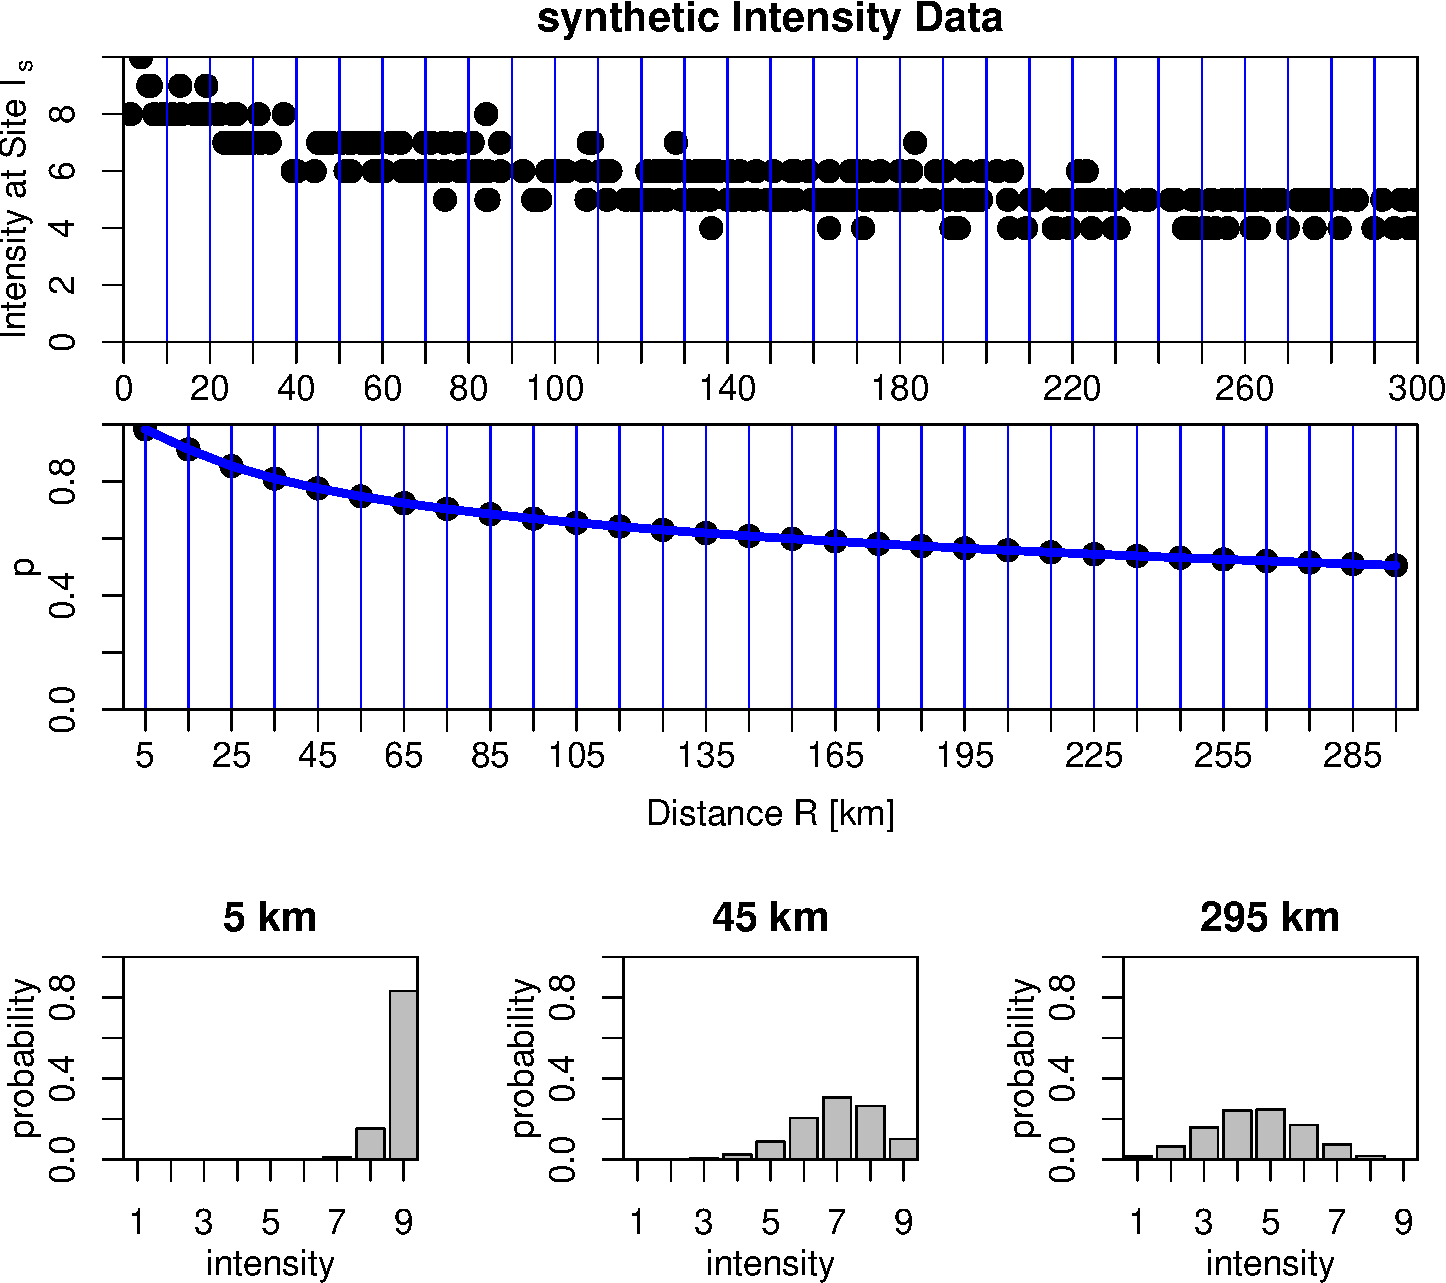
\includegraphics[scale=0.6]{Figures/example.pdf}
		\rule{35em}{0.5pt}
	\caption[Example]{Example of the process of developing groundmotion models. The top figure shows a data set of macroseismic observations. These are discretized into distance bins with a width of 10 km. In each distance bin the abservations are used to update the prior parameter of the Beta distribution. In the middle figure the mean of the posterior Beta distributions is assigned to the middle of the distance bins a smoothing function is used to get values of the p parameter for every distance. The bottom figure shows the probability distribution for different distances once the posterior mean of the Beta distribution is supplied to the binomial distribution.}
	\label{fig:example}
\end{figure}

 
% Chapter 3

\chapter{Sensitivity study} % Main chapter title

\label{Chapter3} % For referencing the chapter elsewhere, use \ref{Chapter1} 

\lhead{3. \emph{Sensitivity Study}} % This is for the header on each page - perhaps a shortened title

\section{Synthetic Data}

Testing the performance of a model is a crucial step in defining new ground motion relationships and should always accompany the process of creating models. Especially in seismic risk evaluation one is interested how different parameters influence the reliability of the result. A sensitivity study evaluates the performance and gives the user a guide how to use a model in real life applications, how to quantify possible errors and which parameter should be given a higher priority in order to minimize uncertainties efficiently.
To test the performance of the model from \cite{Rotondi2004} first, a series of tests is performed on a set of synthetic intensity data. The synthetic data is constructed by sampling 700 distance values uniformly over a range of 300 kilometres. In order to calculate corresponding intensity values the model of \cite{Koveslighety1906} is used together with an epicentral intensity($I_0$) of IX:
\vspace{0.1cm}
\begin{equation}
\Delta I = a * log_{10}\left(\dfrac{d_h}{h}\right) + a * b * log(d_h -h)
\label{eqn:koveslighety}
\end{equation}

\begin{figure}[!htpb]
	\centering
		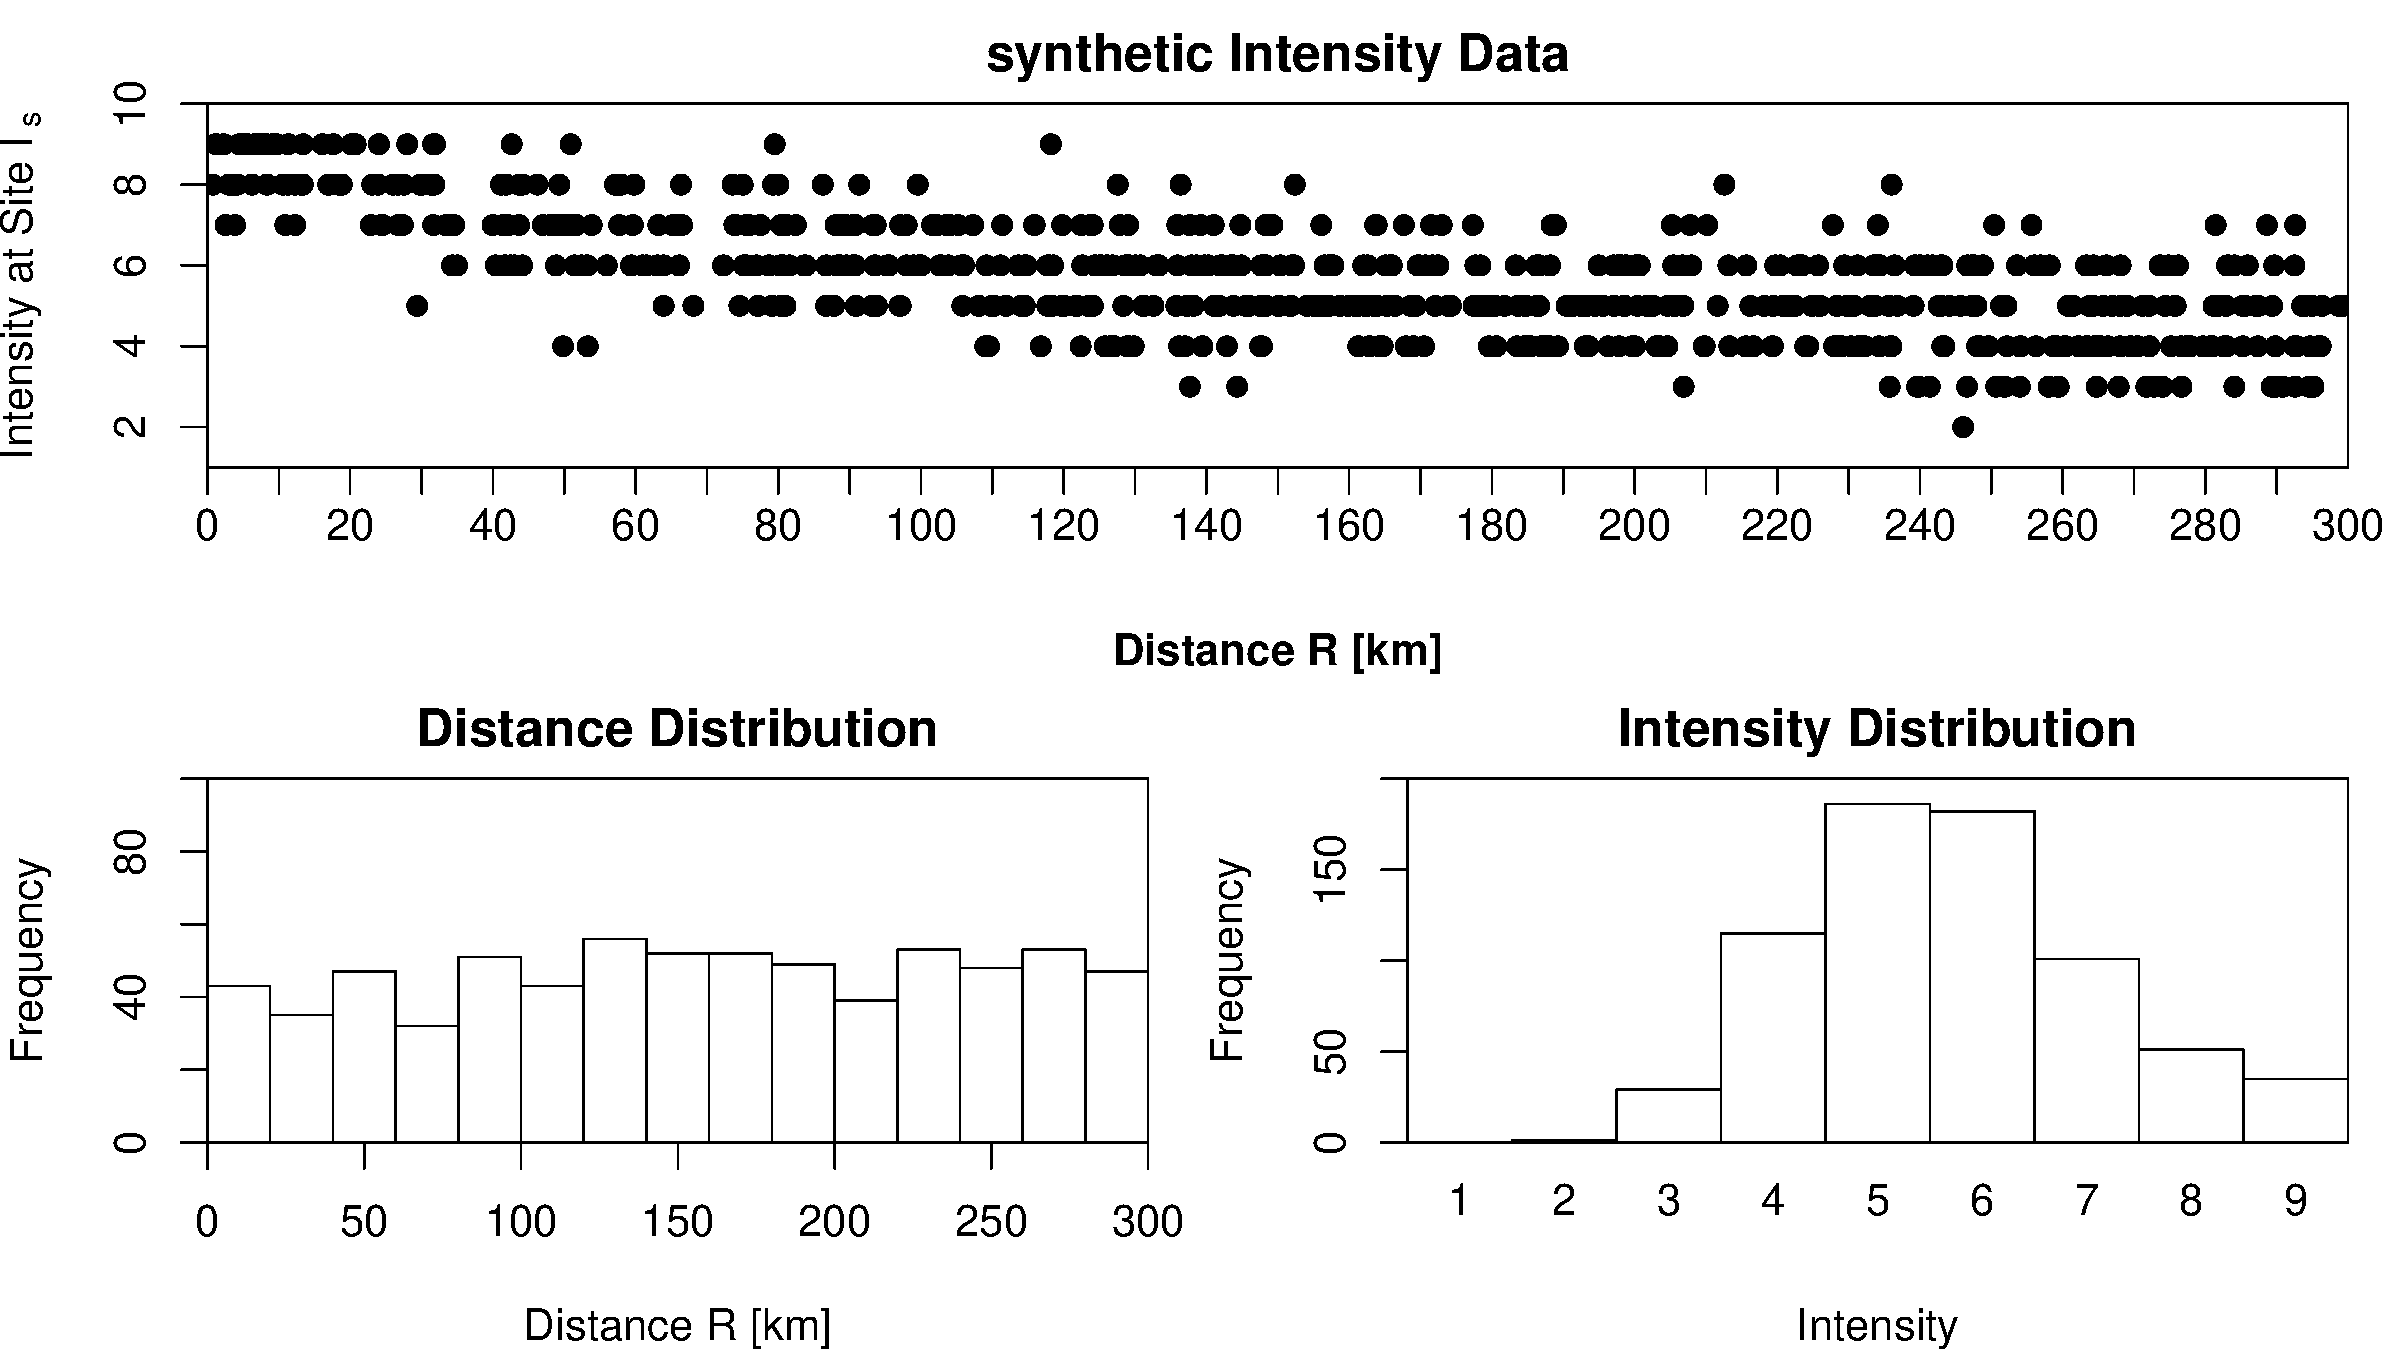
\includegraphics[scale=0.33]{Figures/dataDistro.pdf}
		\rule{35em}{0.5pt}
	\caption[synthetic data]{Synthetic data according to equation \ref{eqn:koveslighety}. Distance values where uniformly sampled over a distance range up to 300 kilometers.}
	\label{fig:dataDistro}
\end{figure}

where
$d_h = \sqrt{R^2+h^2}$ is the hypocentral distance of the earthquake, h = 10km is the depth of the earthquake hypocentre, $a$ = 3 is a factor for the geometrical spreading of seismic waves and $b = 0.002 km^{-1}$ is a parameter that accounts for the anelastic dissipation \citep{stromeyer2009attenuation}. To attain whole numbers the results of equation \ref{eqn:koveslighety} are rounded. As prior distribution a uniform distribution over the range between 0 and 1 is used corresponding to the hyperparameters of the Beta distribution $\alpha = \beta = 1$.



To estimate the prediction performance the mode of the binomial distribution for each distance bin is used in order to forecast intensities. The mean absolute error between predicted and synthetic intensities is the measure for the prediction ability.

\section{Data Size}

One important and very limiting factor for generating new ground motion models is the amount of data that is available. Depending on the region one might encounter scenarios where rich catalogues of past seismicity are available or just a sparse set of observations. To test the behaviour of the model in these different environments the synthetic data has been randomly partitioned into subsets of stepwise increasing number of observation, thus simulating the effect of different catalogue sizes. To estimate the model's performance a 10-fold cross-validation procedure is adopted to estimate the training error (in-sample error) as a measure of how well the model can approximate the data and the cross-validation error (out-of-sample error) which examines the performance on data that was not used in estimating the parameters of the model. Also it is a very easy way to qualitatively diagnose whether the model is suffering from bias or variance. Bias means the model's ability to approximate the target function that has generated the data. Variance quantifies how sensitive this estimate is to a specific subset of the data.  In a high bias case fit and cross-validation error would rapidly approach each other and remain equal on a high level. This means that adding more data does not improve the models performance since the model that is used to fit the target function can only approximate it poorly. It is a case of underfitting. Conversely, in a high variance scenario there is a gap between fit and cross-validation error but the cross-validation error still decreases with more data. This situation corresponds to overfitting.\\
 
\begin{figure}[!htpb]
	\centering
		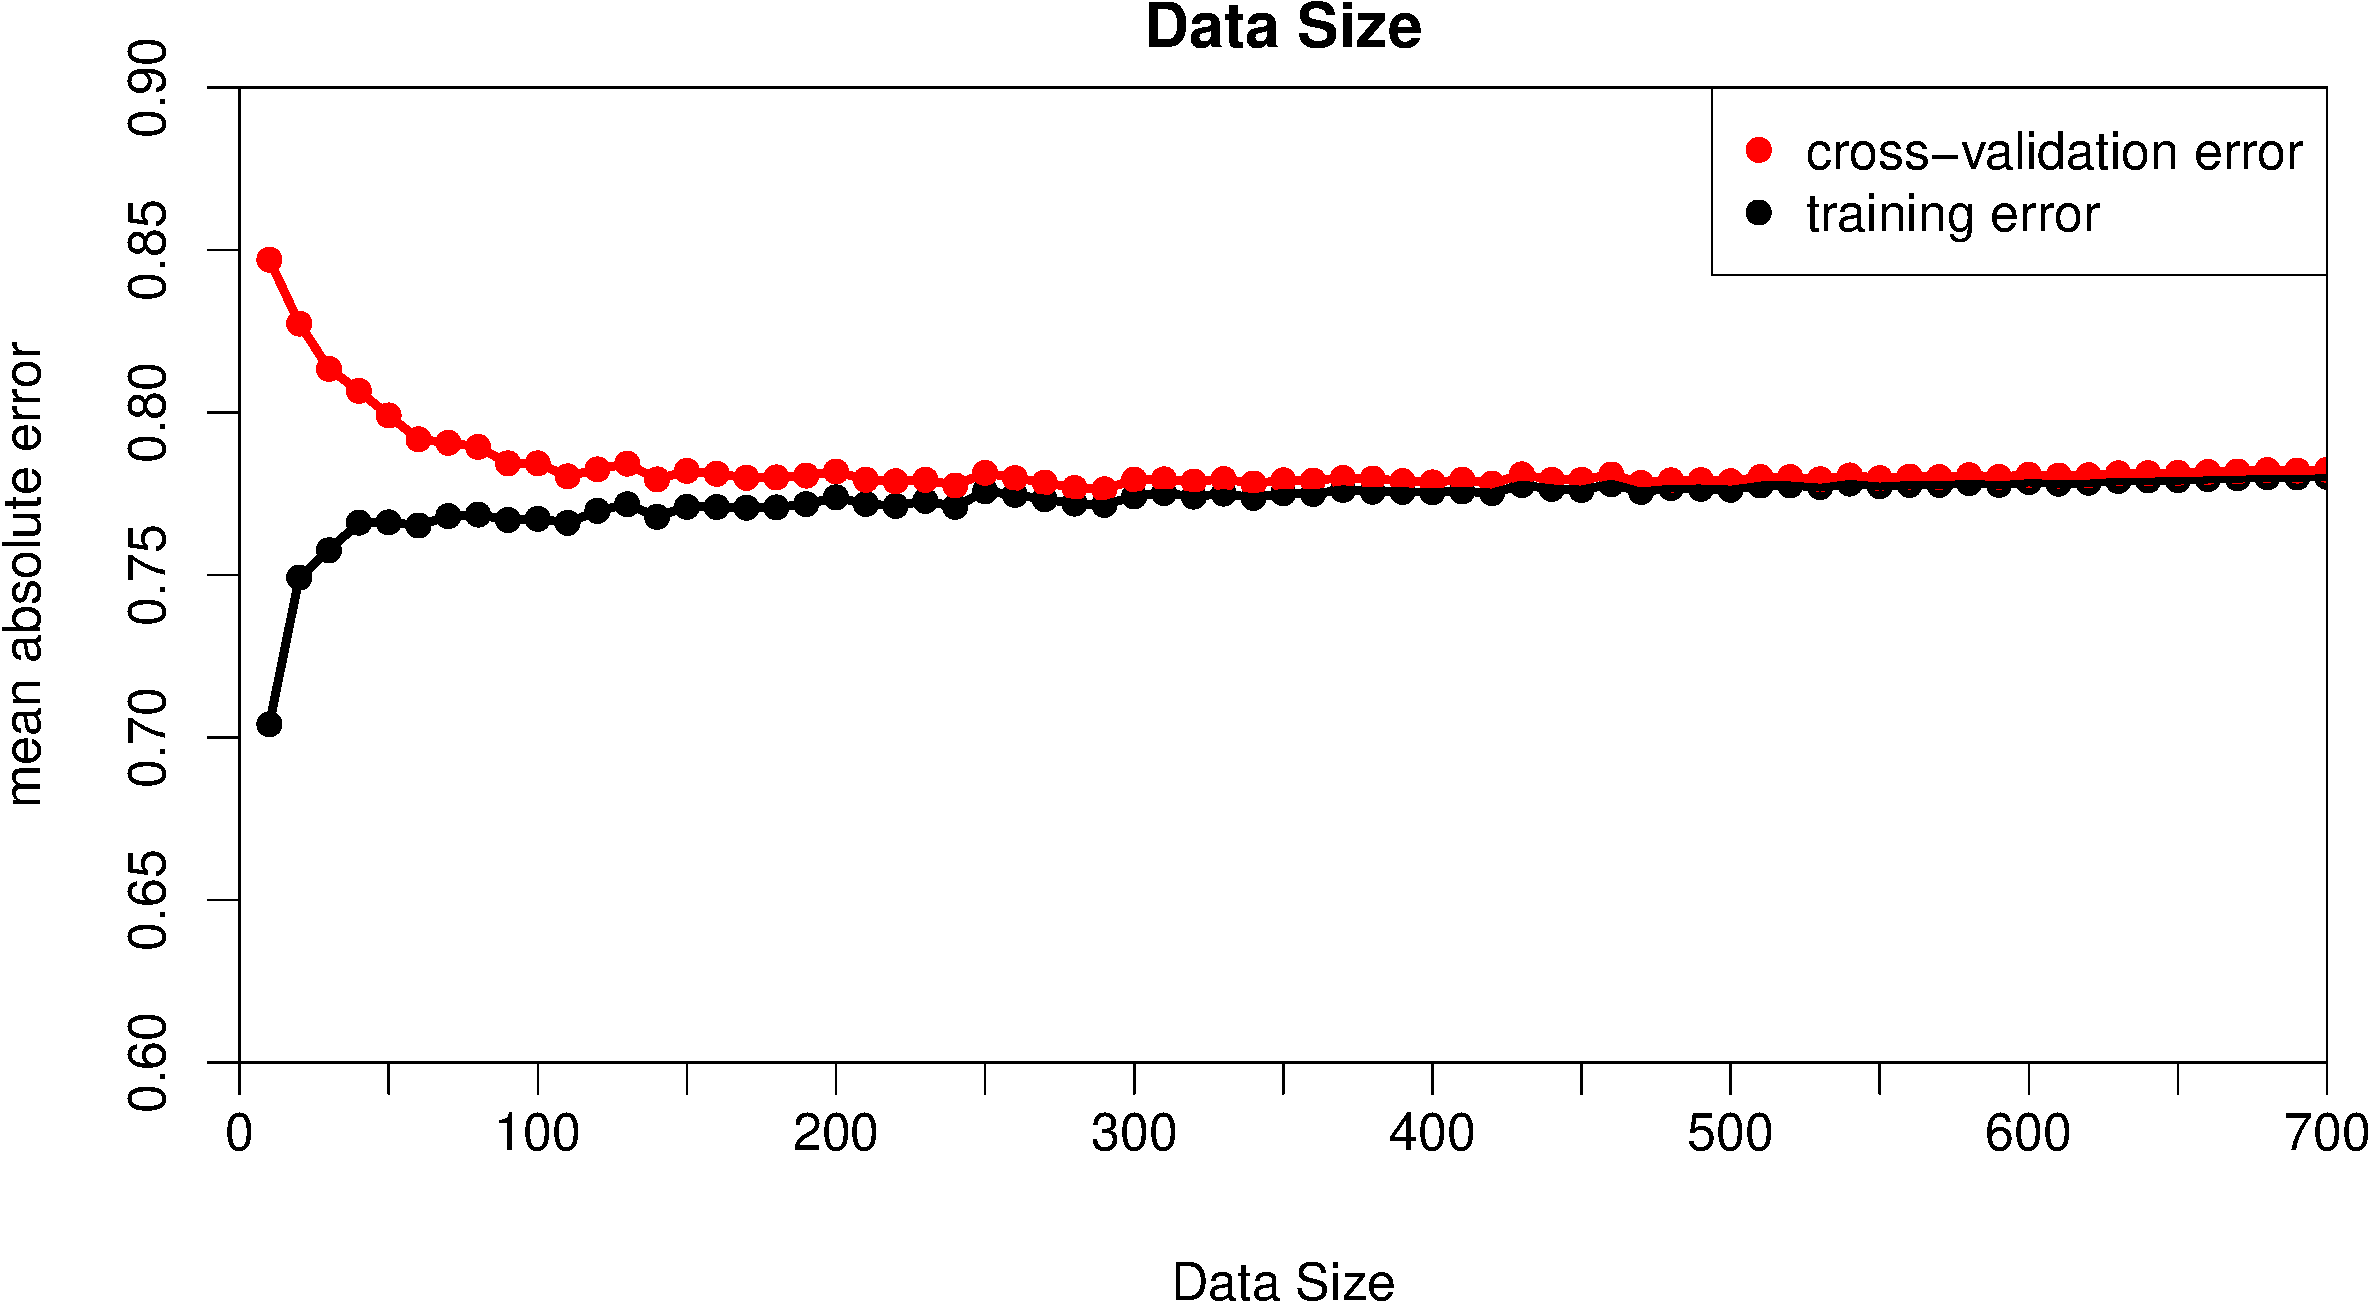
\includegraphics[scale=0.33]{Figures/numberData.pdf}
		\rule{35em}{0.5pt}
	\caption[Data Size]{Data Size}
	\label{fig:data}
\end{figure}

Figure \ref{fig:data} shows the results of this analysis. With a small data set size the cross-validation error is larger than the training error. This means that the trained model does not well generalize to unseen data. Increasing the data set size results in decreasing cross-validation error and increasing training error. Though it becomes harder to replicate all of the training data the model performs better in predicting. At around 500 data samples there is no real difference between cross-validation and training error. 

\section{Quality of the Data}
Another parameter that can heavily influence the computation of new ground motion relationships is the quality of the data. The best algorithm can only perform as well as the used data. To simulate the effect of poor data a Gaussian error with a mean equal to zero and a stepwise increasing standard deviation is added to synthetic data. Since only the isolated effect of poor data should be studied the whole 1000 synthetic observations are used. Because at this data size there is no difference in training error and cross-validation error only the cross-validation error is shown in Figure \ref{fig:noise}.

\begin{figure}[!htb]
	\centering
		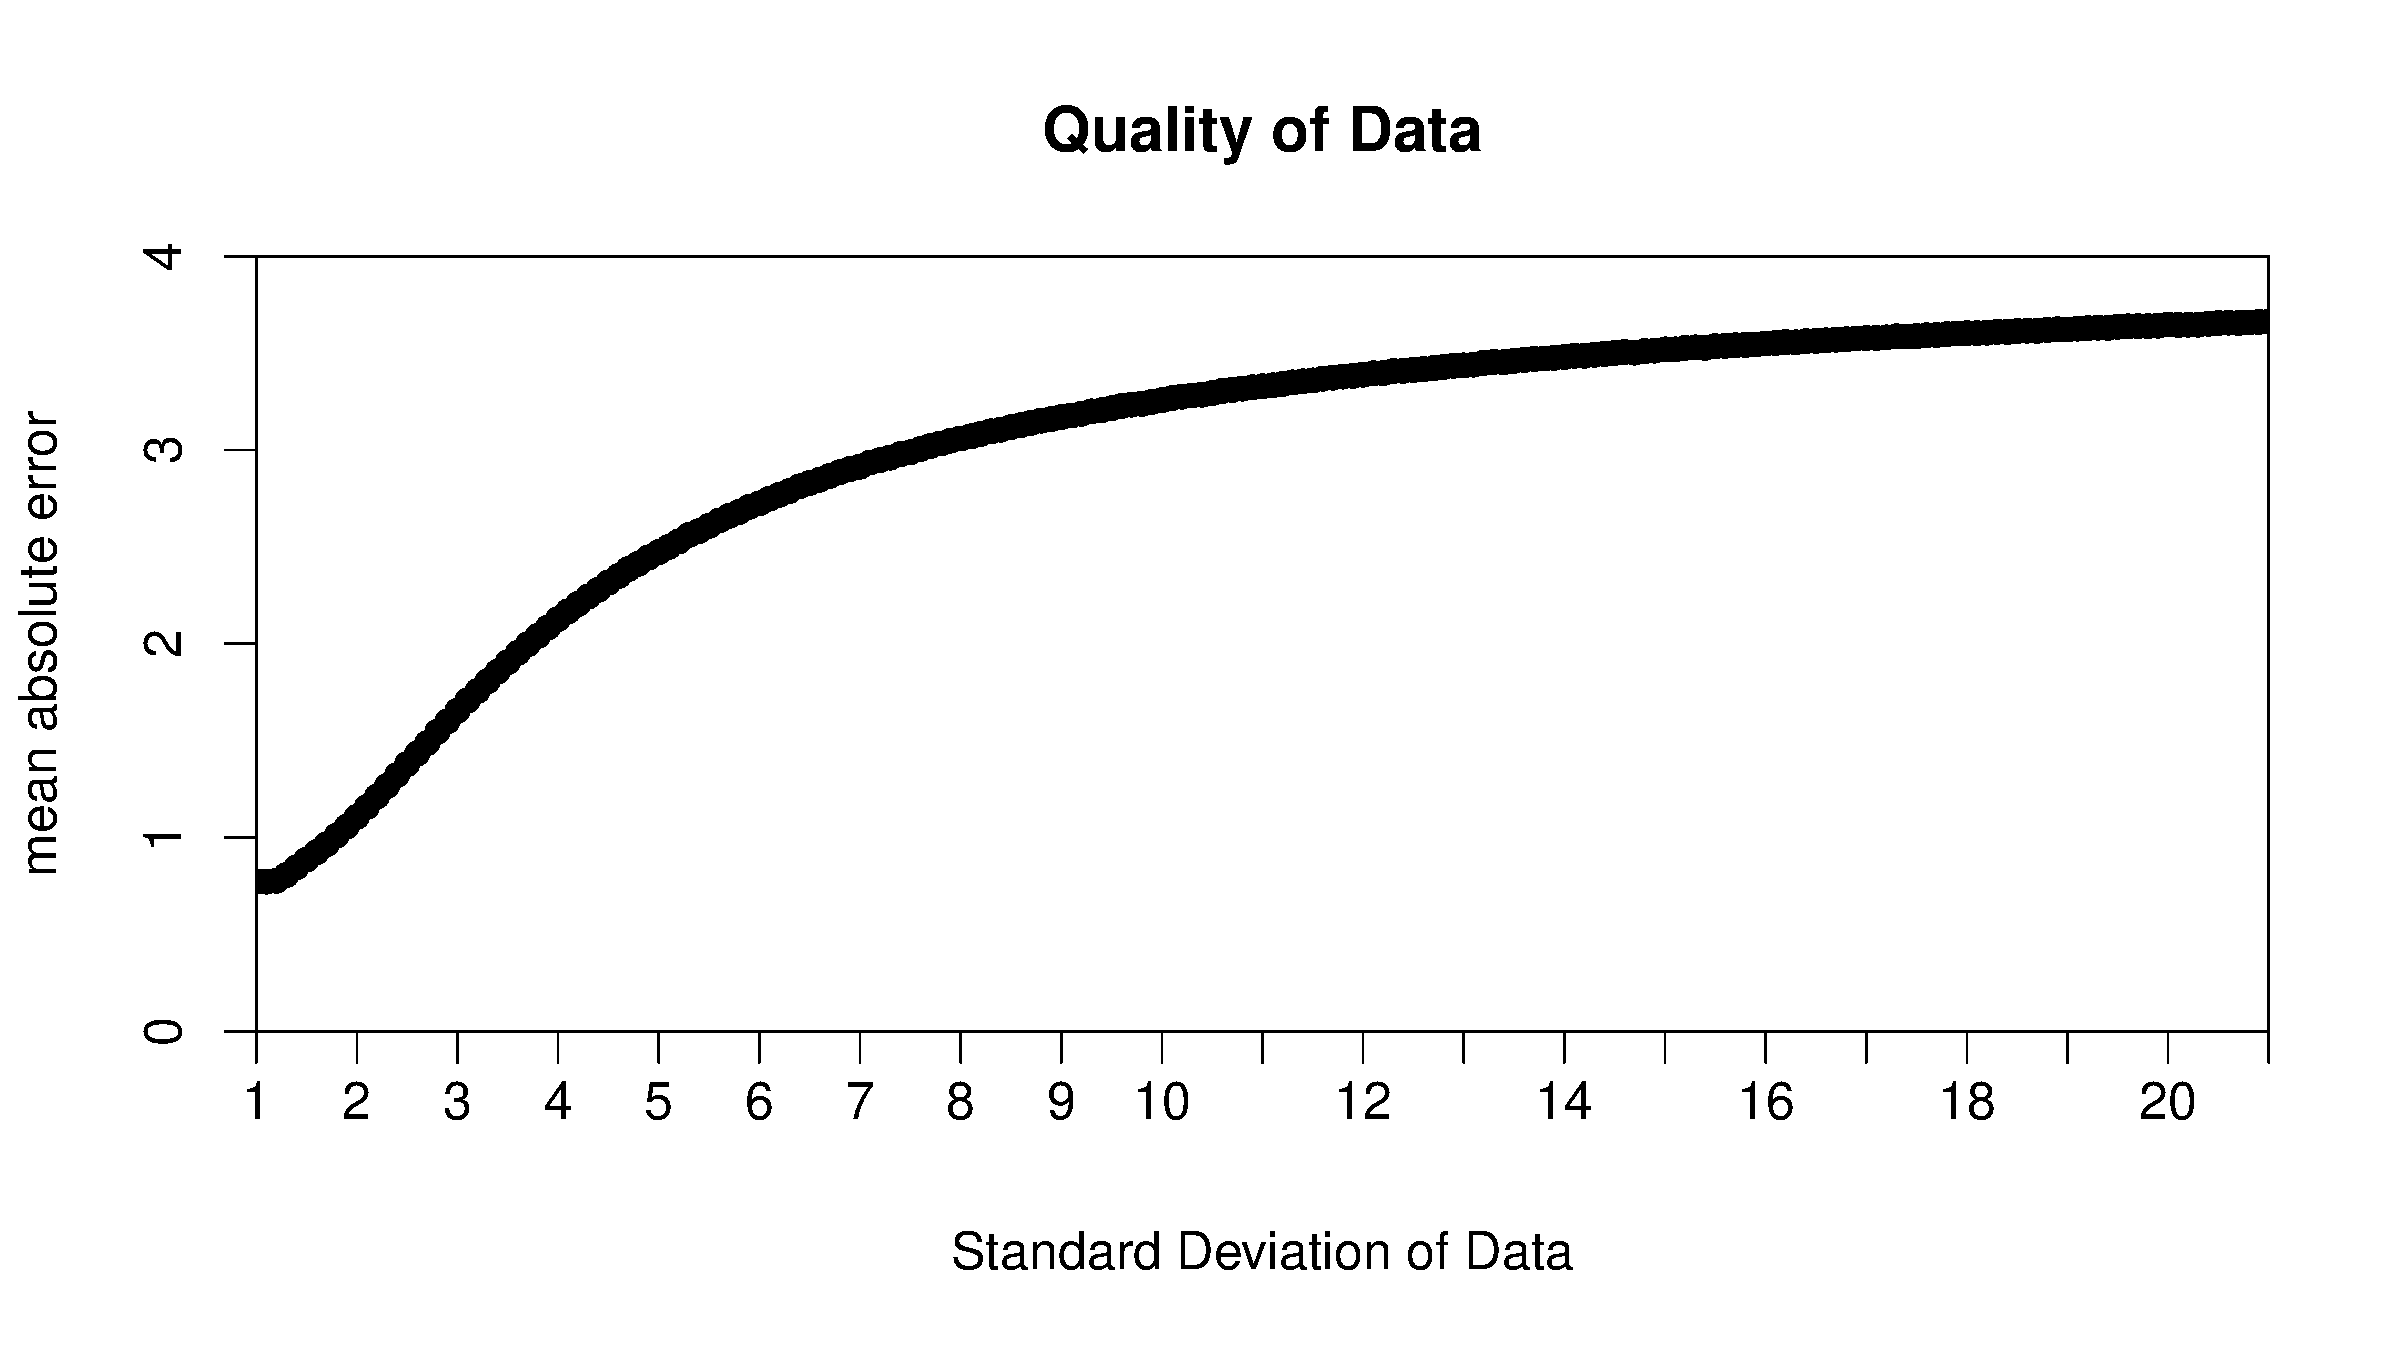
\includegraphics[scale=0.335]{Figures/noise.pdf}
		\rule{35em}{0.5pt}
	\caption[Quality of Data]{Quality of Data}
	\label{fig:noise}
\end{figure}



The mean absolute error increases in a logarithmically fashion with greater noise that is added to the data. This can be explained with the fact that as the noise in the data increases more individual data points take the intensity values of I or IX which are the extremes of the intensity range. This placed an upper limit to the mean absolute error that can be achieved by adding random noise. \\
  
Figure \ref{fig:noiseData} shows the analysis of changing data size and noise level in the data simultaneously. The advantage of more data for the algorithm to learn from seems just relevant for scenarios where there is only a small data set to learn from. Beyond 300 data samples the mean absolute error depends mainly on the level of added noise. This behaviour is exactly what one would expect given that the out-of sample error can be divided into a bias, variance and noise part\citep{LearningFromData}. From the analysis of the influence of data size on the models performance it is known that it suffers from bias. So once enough data samples have been used so that the bias does not change any more the noise level is the only contributing factor.

\begin{figure}[!htpb]
	\centering
		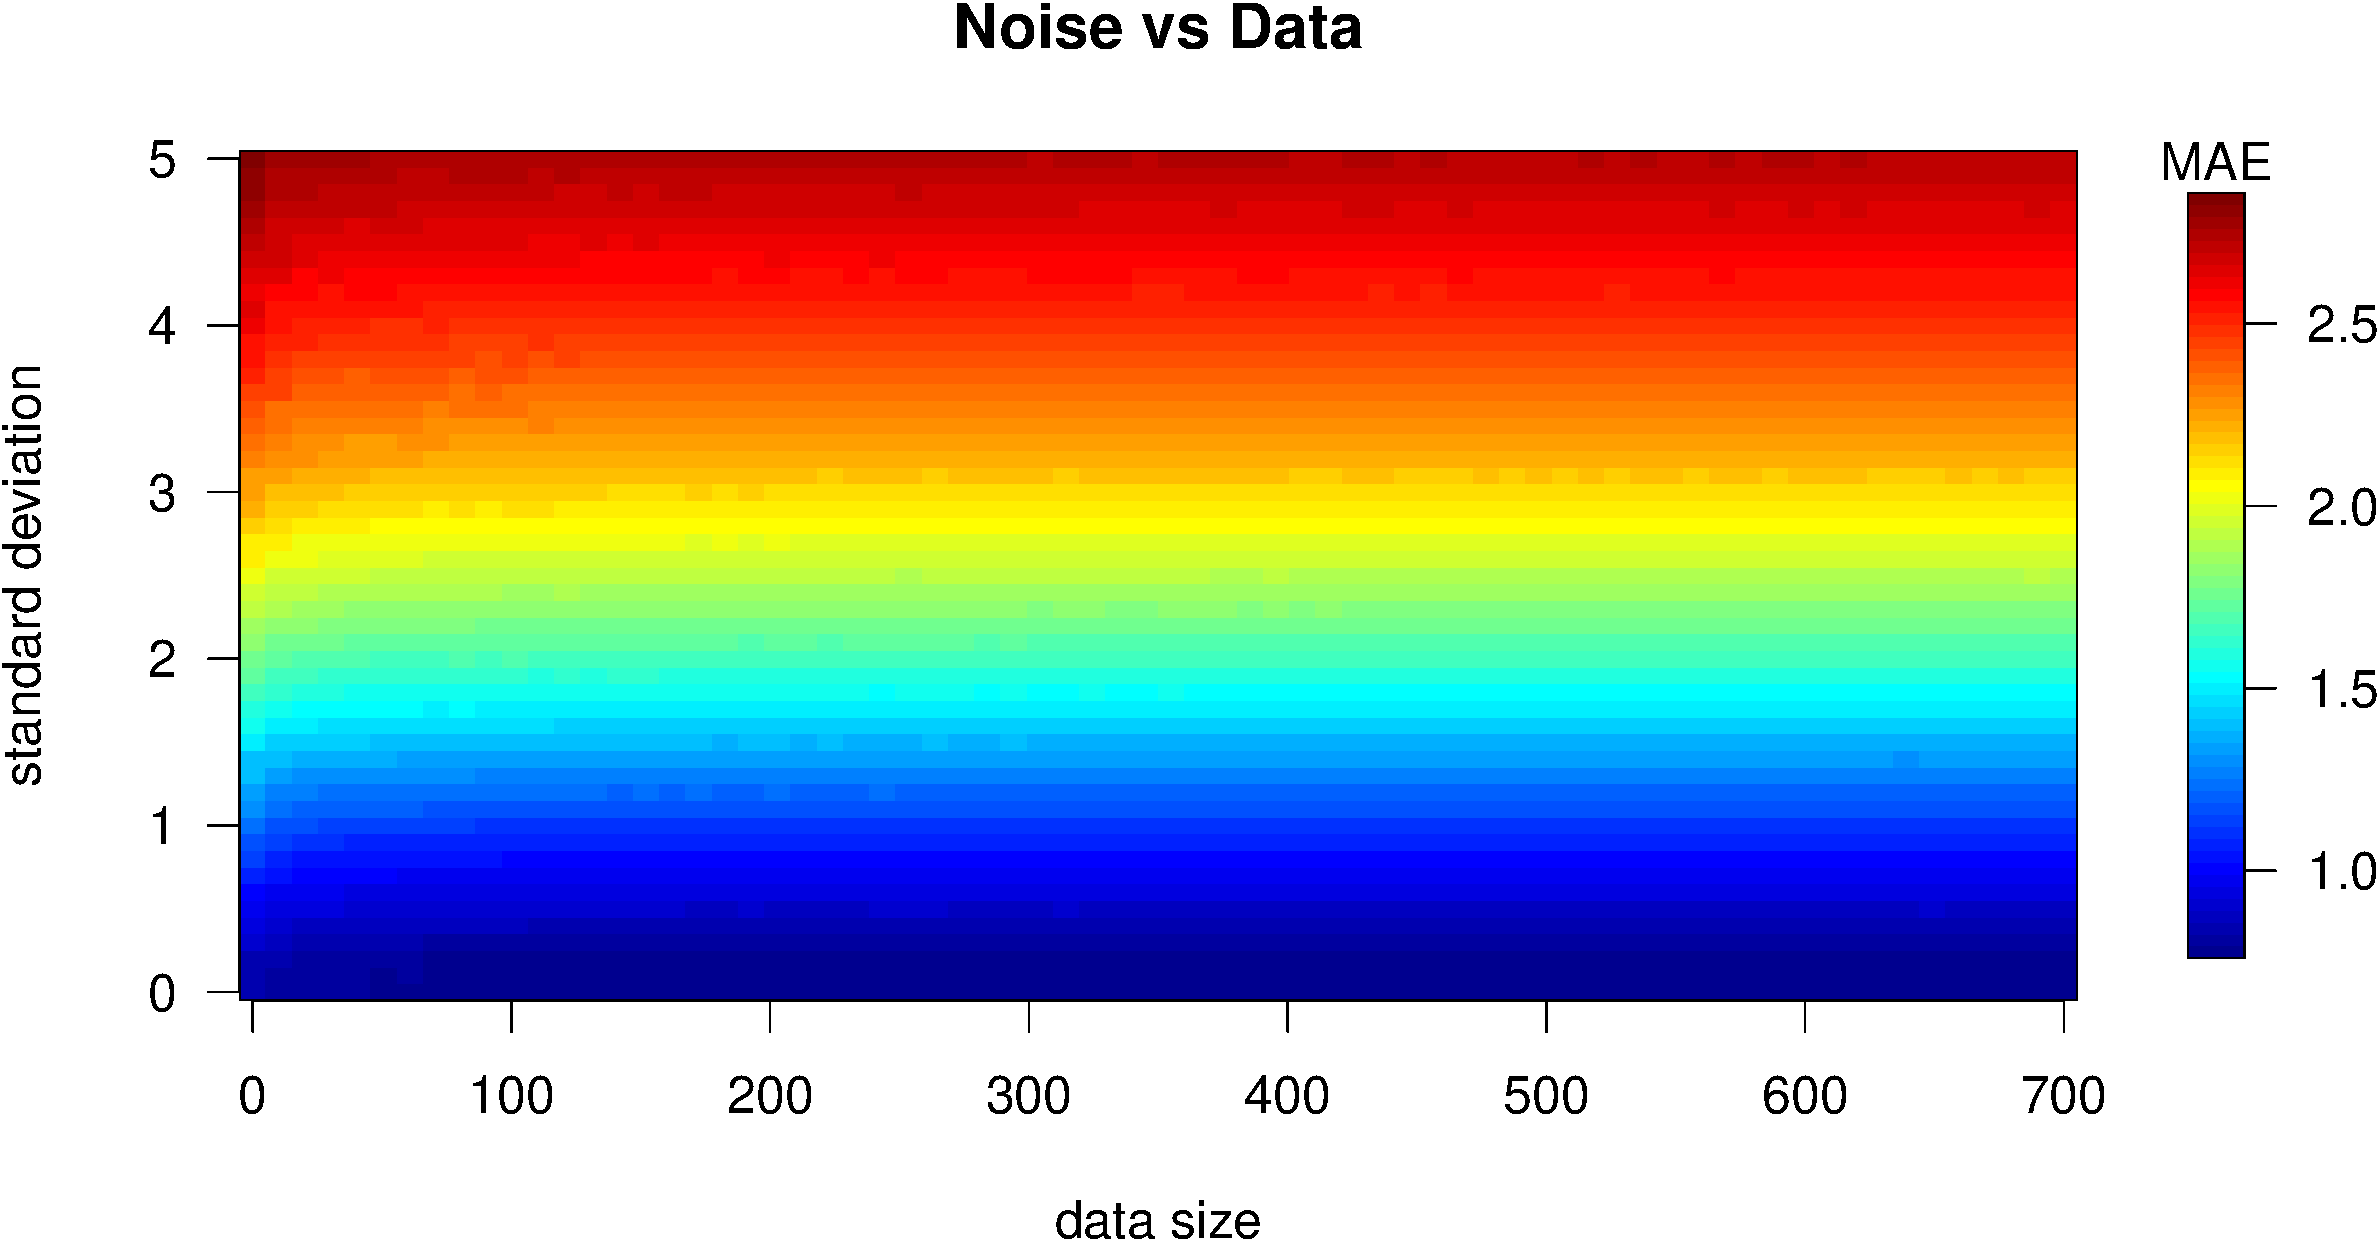
\includegraphics[scale=0.33]{Figures/numberDataNoise.pdf}
		\rule{35em}{0.5pt}
	\caption[Data Size vs Noise]{Data Size vs Noise}
	\label{fig:noiseData}
\end{figure}
\section{Discretization}

One special property of the model by \cite{Rotondi2004} is the discretization of the data into bins of distance. This is necessary since the approach of modelling the intensity distribution by a binomial distribution can only approximate the intensity decay for a certain distance range. To jointly model the intensity distribution an it's dependence on distance one would have to use more advanced techniques like copulas. This subdivision in discrete distance bins is therefore a compromise between enough data per bin to estimate the parameter p of the binomial distribution with great accuracy and enough bins spanning the whole range of site to source distance in order to have a thorough support for the smoothing function. The whole data set of 700 synthetic observations is used and the cross-validation error is chosen as measure of prediction performance. 

\begin{figure}[!htpb]
	\centering
		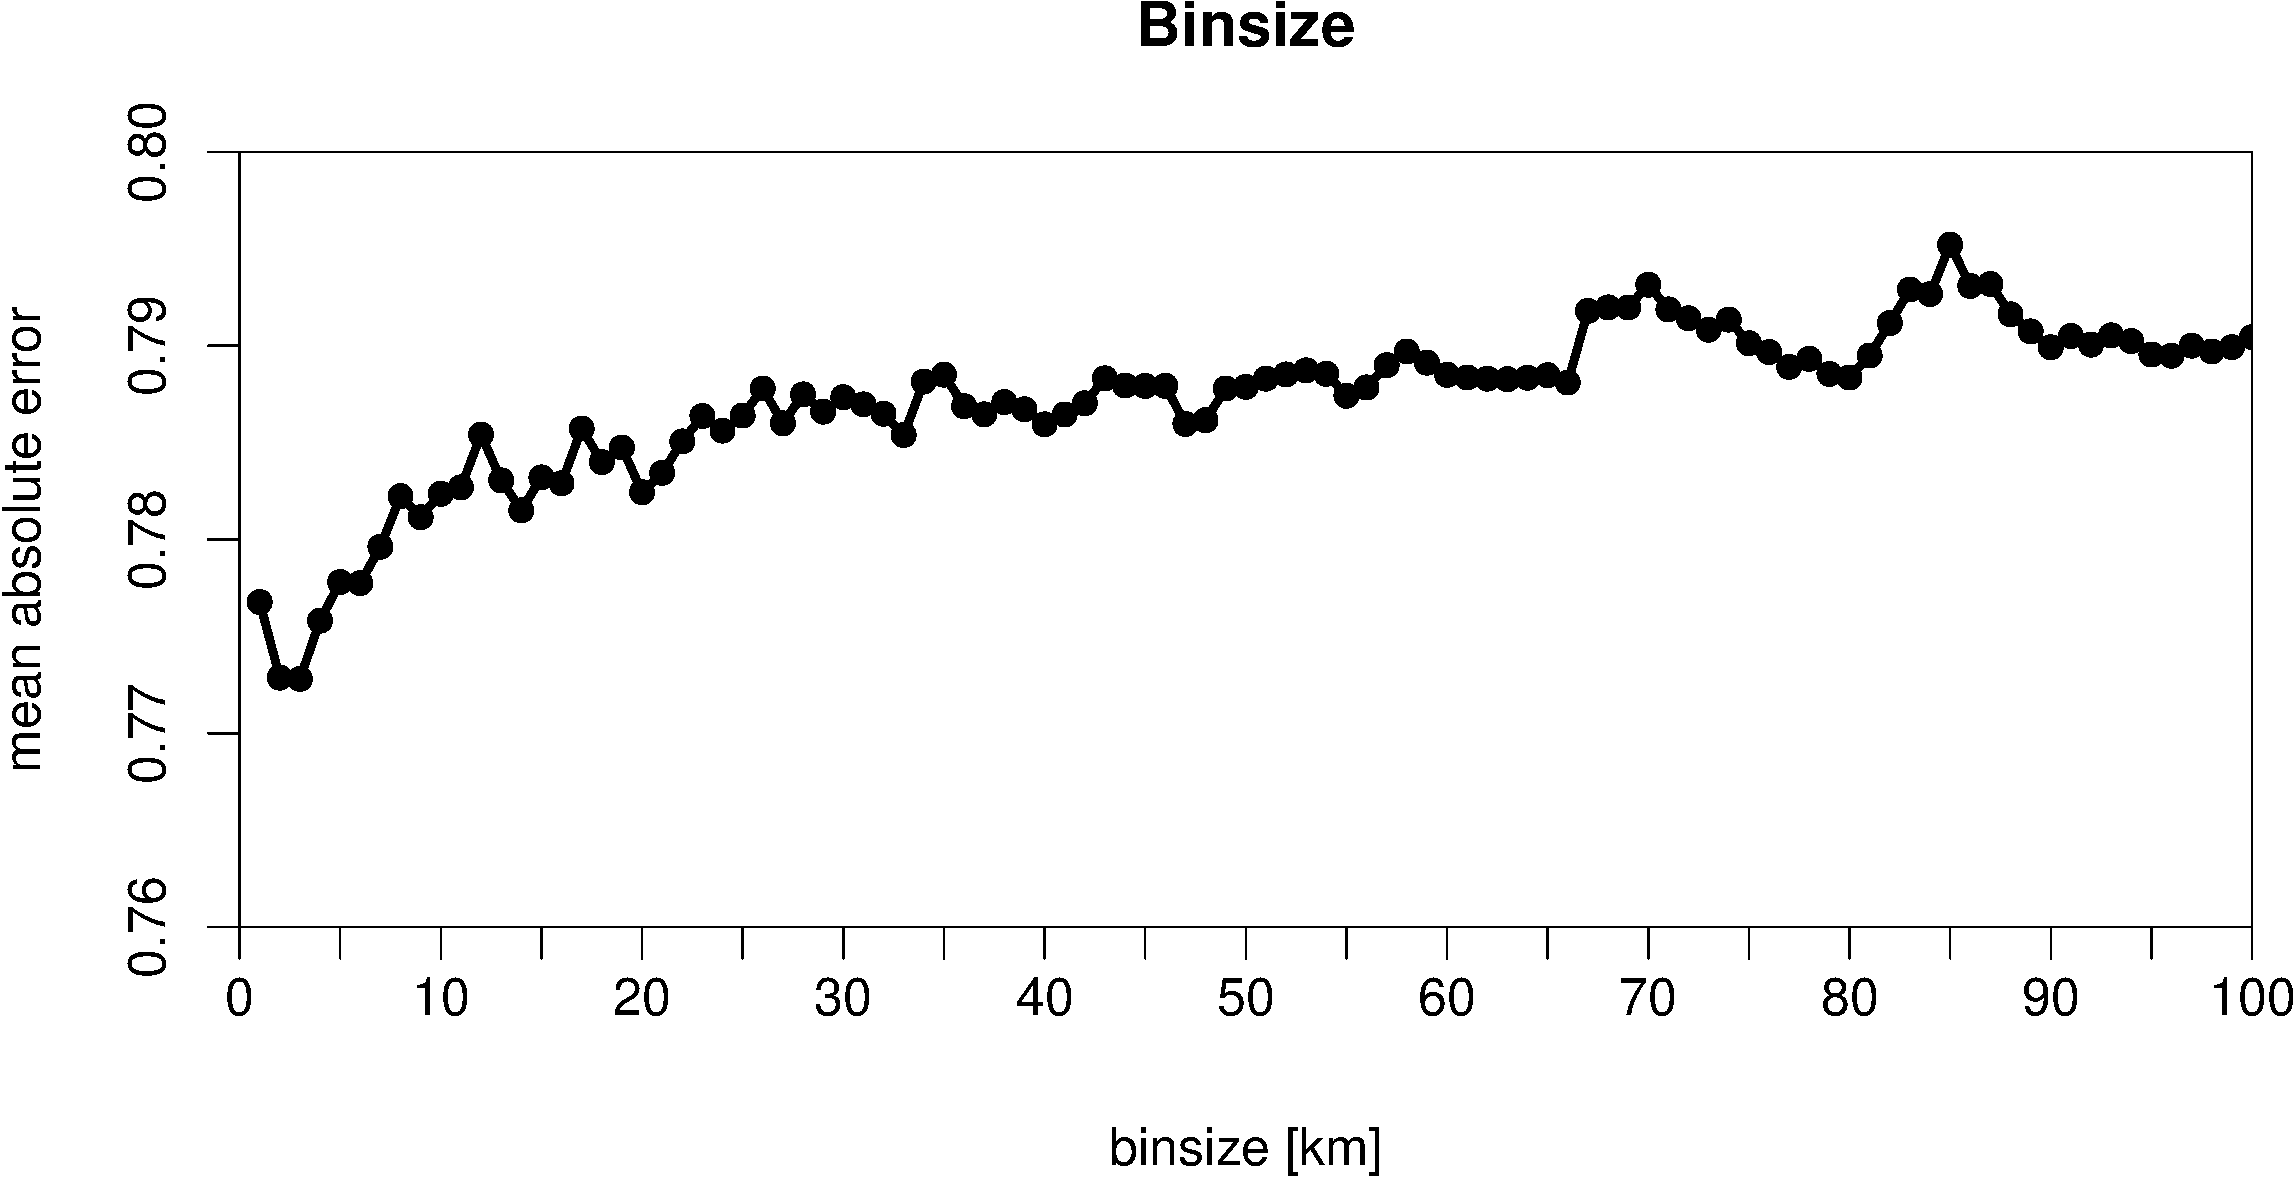
\includegraphics[scale=0.33]{Figures/binsize.pdf}
		\rule{35em}{0.5pt}
	\caption[distance bin size]{distance bin size}
	\label{fig:binsize}
\end{figure}

Figure \ref{fig:binsize} shows the result of a stepwise increase in the width of the distance bins. The lowest mean absolute errors are achieved with bin sizes of 2-3 km. After this point the error increases logarithmically with larger bin widths. It should also be noted that the maximum differences between different bin sizes, and thus the influence of the choice of one particular bin size on the overall error, are relatively small.\\
Figure \ref{fig:binsizeData} shows the results of changing bin size and data size simultaneously. Larger bin sizes affect the mean absolute error on small data sets more heavily than on larger data sets. A general trend of lower errors for smaller bin sizes can be found although this influence is decreased with larger data set size.\\

\begin{figure}[!htpb]
	\centering
		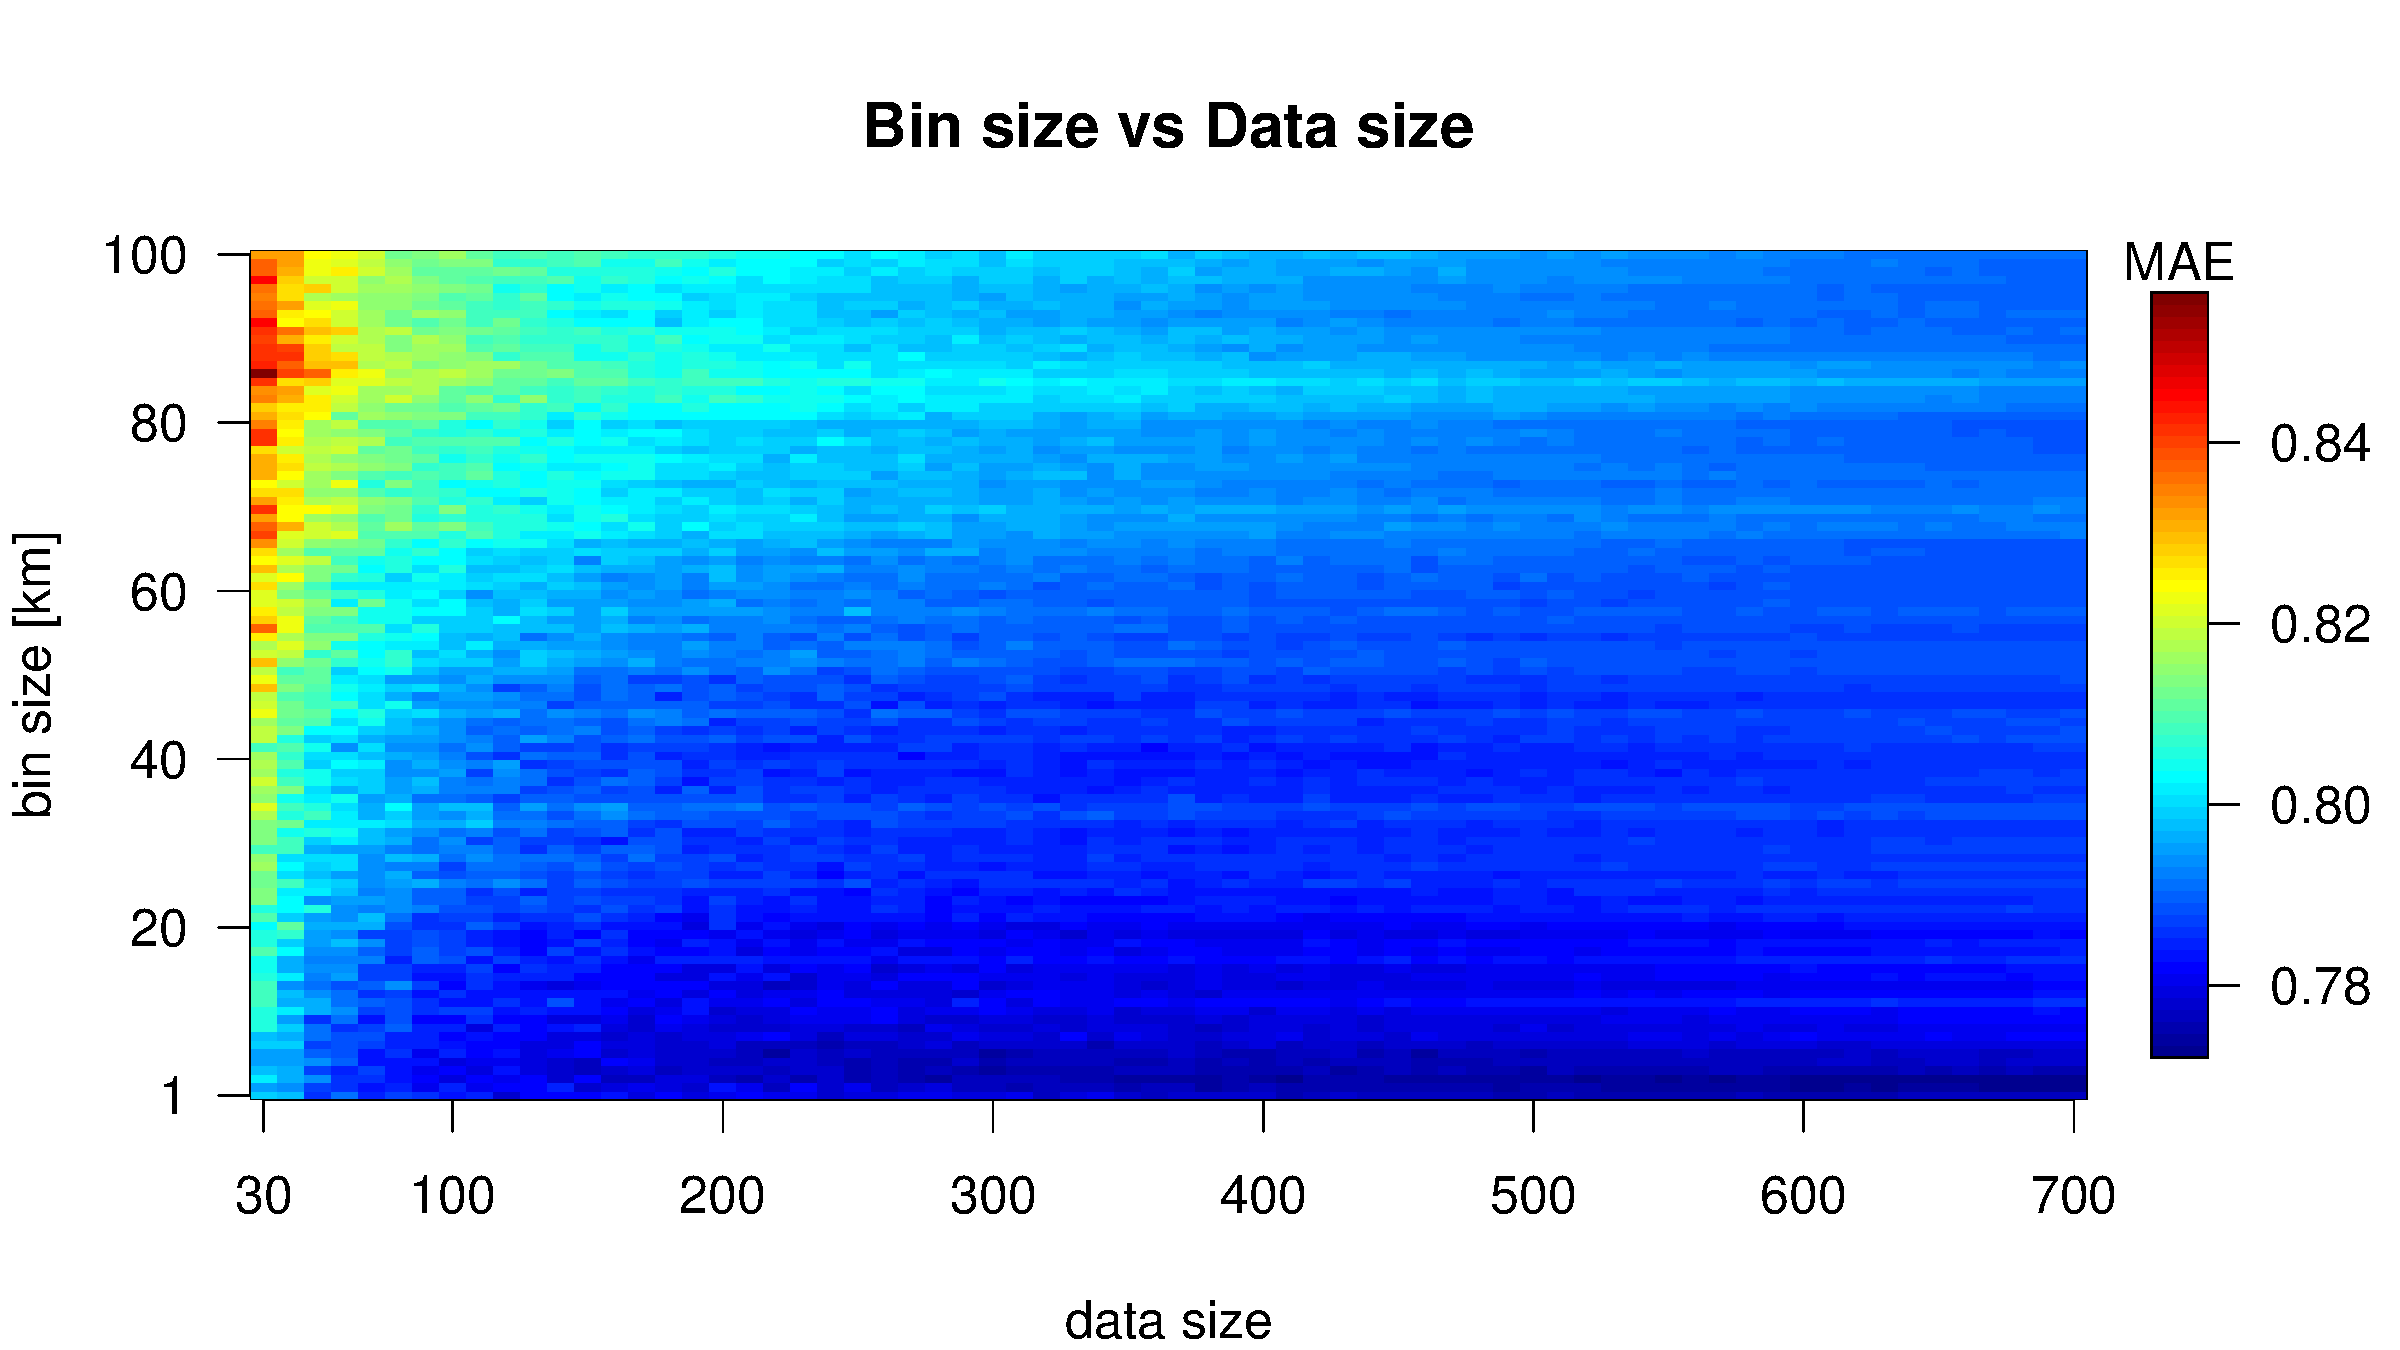
\includegraphics[scale=0.33]{Figures/binsizeDatasize.pdf}
		\rule{35em}{0.5pt}
	\caption[Data Size vs binsize]{Data Size vs binsize}
	\label{fig:binsizeData}
\end{figure}

\section{Sample Bias}
The distribution of samples in distance has up until now be modelled by a uniform distribution. Following the effect of a biased coverage of the distance range on the performance of the model is studied. Therefore, additional to the uniform distance distribution, three distance distributions corresponding to scenarios where the majority of data is available in a middle, a near and a far distance range, respectively, are used to generate synthetic intensity data. The cross-validation error is used as an estimate of the prediction performance.\\
Figure \ref{fig:sampleBias} shows the corresponding distance distributions and the result of this analysis. The lowest mean absolute errors are produced by a uniform distance distribution. The near and middle range distributions differ for a small data size with the near range distribution performing slightly better. But both approach similar error values with larger data sets. The far range distance distribution performs the worst. This is due to the non-linear nature of the intensity decay where most of the information is in the near distance range in which the intensities attenuate more strongly.

\begin{figure}[!htpb]
    \centering
		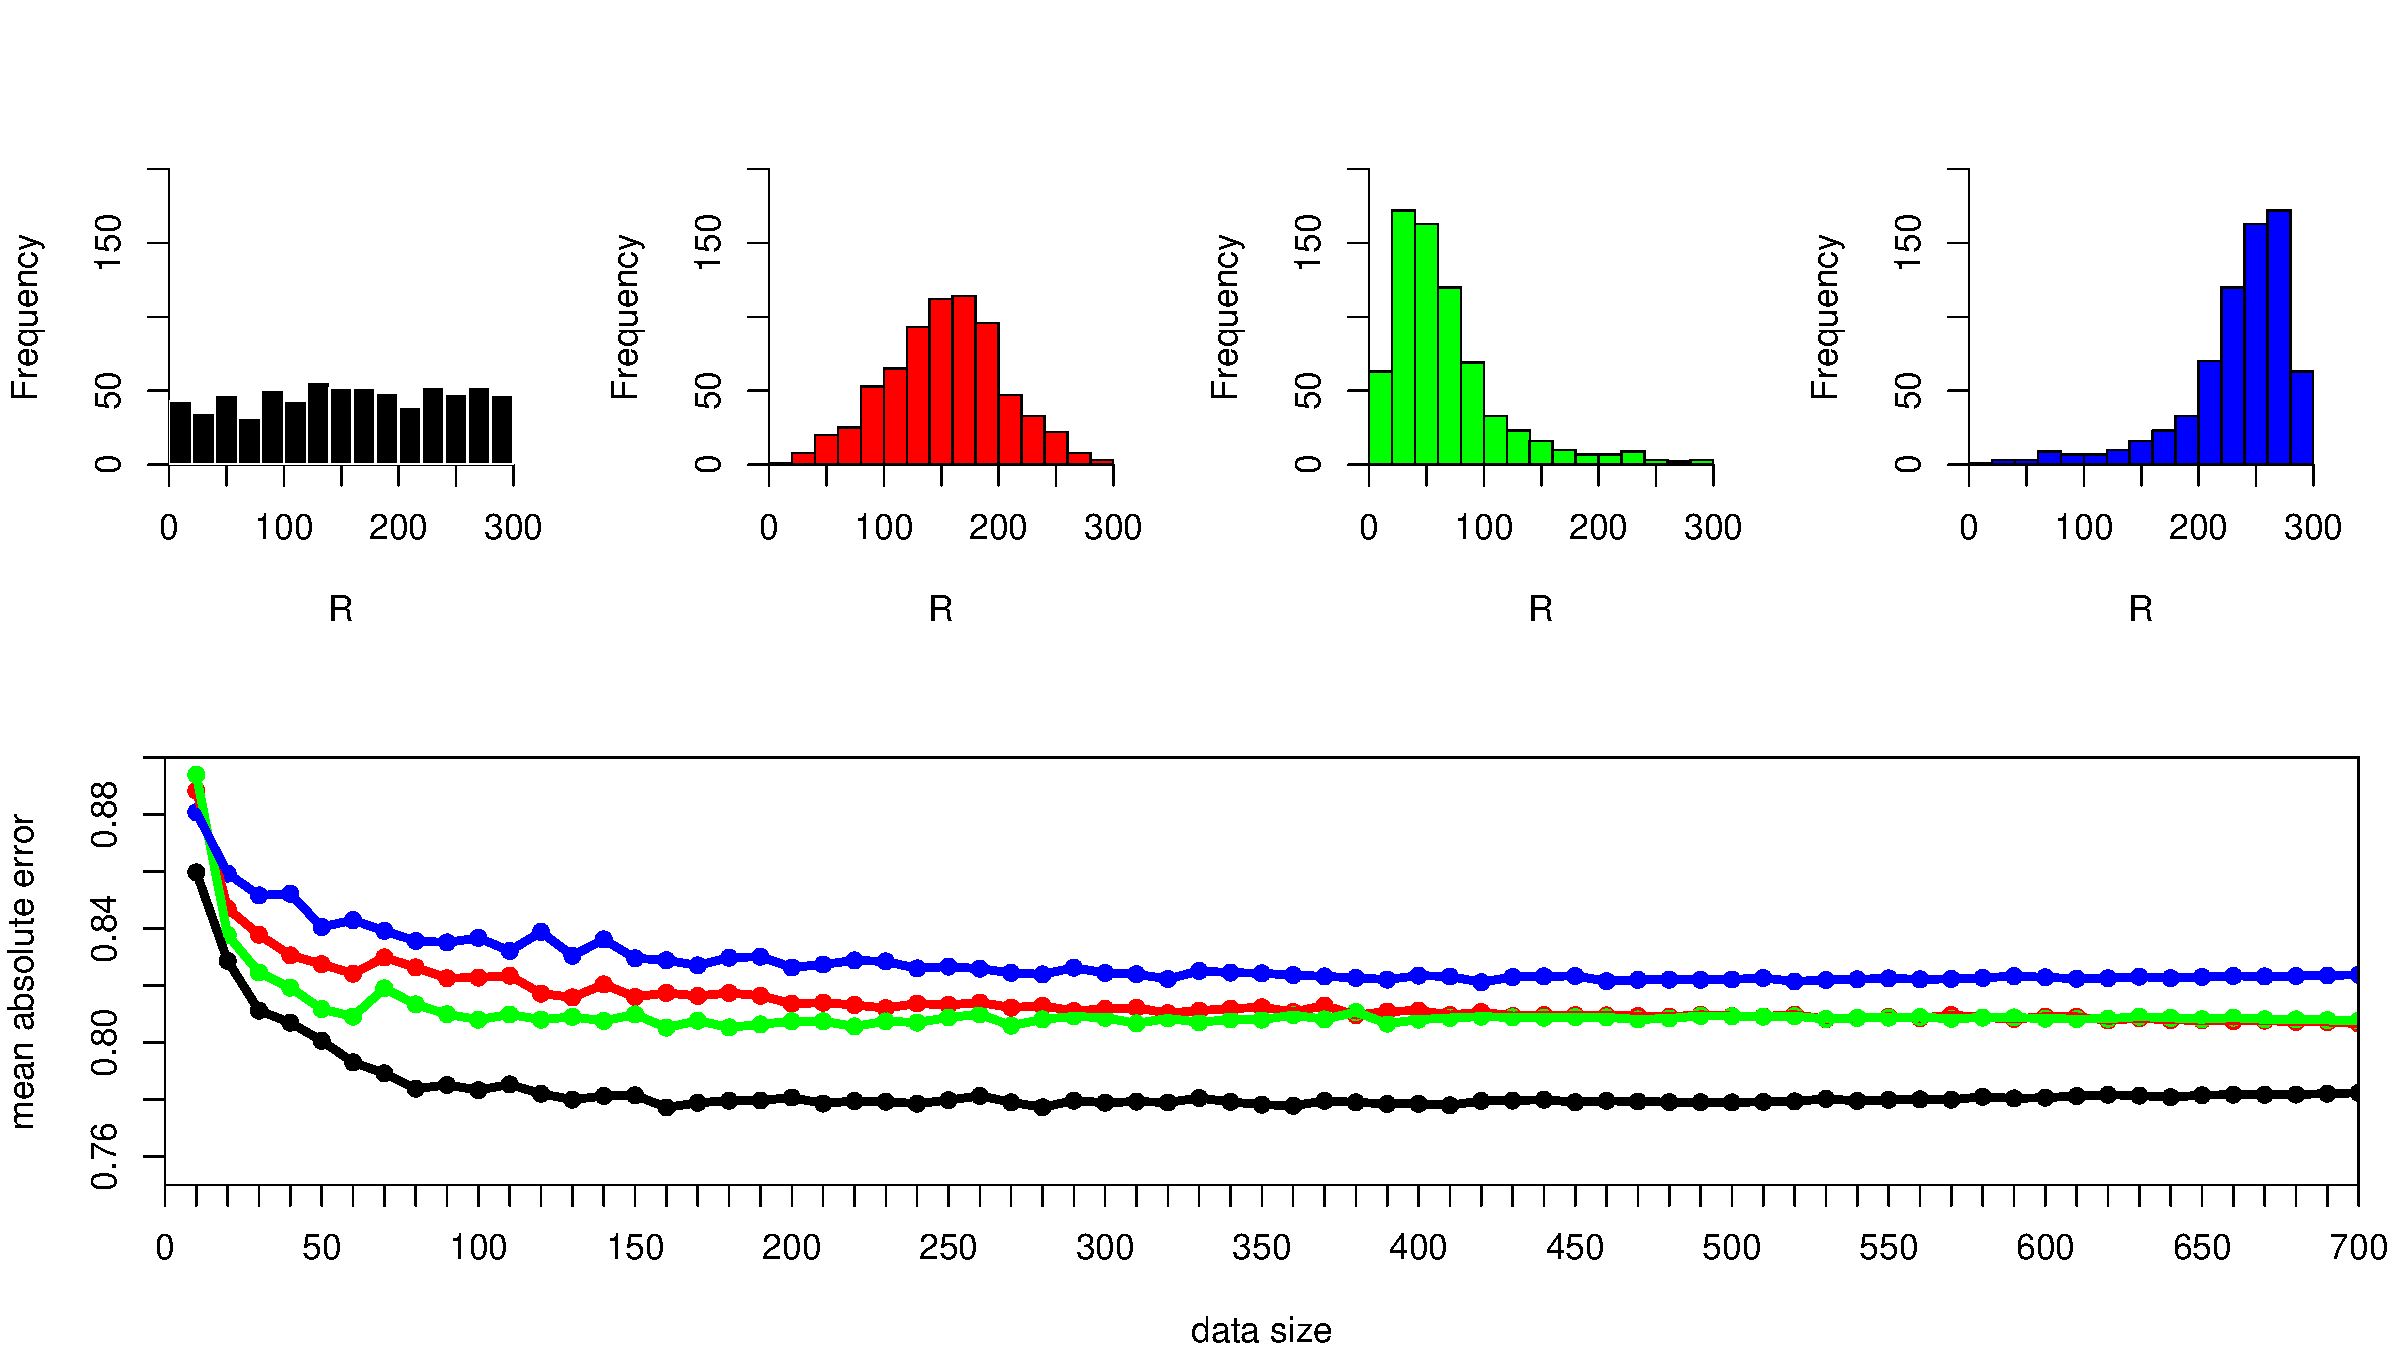
\includegraphics[scale=0.33]{Figures/sampleBias.pdf}
		\rule{35em}{0.5pt}
	\caption[Sample Bias]{Sample Bias}
	\label{fig:sampleBias}
\end{figure}



\section{Choice of Prior Distribution}

A special advantage of a Bayesian approach to ground motion modelling is the possibility to incorporate expert knowledge through the prior distribution. This can be thought of as a start value in a grid-search algorithm where a good start value decreases the number of iterations to find a local and possibly global minimum in the error function. The influence of different prior distribution (table \ref{table:prior}) on the modelling process should be shown. These are a modified version of a prior that \cite{Tsapanos2002} use to compute the hazard for Japanese cities, a uniform distribution, two distributions where the mean decreases linearly and exponentially with distance, respectively, and a distribution that uses the prior knowledge of the already existing IPE by \cite{Koveslighety1906}.\\
The challenge here is that a prior distribution in term of the p parameter and not as intensities given a specific distance is needed. Given that some prior knowledge is available in form of an IPE this can be constructed with the help of the update rules for the hyper parameter $\alpha$ and $\beta$ (Eqn:\ref{eqn:updatehyper}). Since no prior values of $\alpha$ and $\beta$ can be updated these values become zero so that:

\begin{equation}
\alpha = \sum^N_{n= 1} i_s \hspace{2cm} \beta = \sum^N_{n= 1} (I_0 - i_s)
\label{eqn:updatehyperPrior}
\end{equation}

Letting N be equal to 1 this becomes:

\begin{equation}
\alpha = i_s \hspace{2cm} \beta = (I_0 - i_s) = \Delta I
\label{eqn:updatehyperPrior}
\end{equation}

It should be noted that it is not in the scope of this thesis to give a full hands-on tutorial in how to choose a prior distribution for the algorithm of \cite{Rotondi2004}. The aim is to show the influence that a prior can have on the computation. It should also be stressed that a prior distribution in a Bayesian framework acts as a kind of regularization term and it is therefore not advisable to tune the prior distribution so that a minimal error is achieved. A prior should quantify expert or domain knowledge and has to be "naive". \\
Figure \ref{fig:priorMeans} shows the attenuation of the prior distributions' means with increasing distance and three visualizations of the full distribution for distances of 10, 150 and 300 kilometres, respectively. An animation can be found in the electronic supplement: \href{https://github.com/silvioschwarz/master-thesis/tree/master/Masterarbeit/gif/plot.gif}{Animation}.\\
Figure \ref{fig:prior} shows the influence that the different prior distributions have on the mean absolute error with increasing data set size. The difference between the prior distributions is the amount of data it is needed in order for the error to converge to a point where it does not decrease any more. This comes from the fact that the influence of the prior on the learning process is decreased with more data samples. Thus, even a prior that is far of as a starting point of the distribution that is in the data can be overcome by more data samples.

\begin{table}[!htpb]
  \centering
       % \small
       % \setlength\tabcolsep{2pt}
%\setlength\extrarowheight{15pt}
%\def\arraystretch{5pt}
\begin{tabular}{|c|c|c|c|c|}
  \hline
prior & $\alpha$ & $\beta$ & $\mu$ & $\sigma$ \\
\hline 
 \rule{0pt}{7ex}\cite{Tsapanos2002}& $\left(\dfrac{1}{1+\dfrac{R}{60}}\right)^{1/I_0}$ & $1 - \alpha$ & $\dfrac{\alpha}{\alpha +\beta}$ & $\dfrac{\alpha \beta }{(\alpha+\beta)^2(\alpha+\beta+1)}$ \\[5ex]\hline
 \rule{0pt}{7ex}\cite{Koveslighety1906} & $I_s^{Koveslighety}$ & $\Delta I^{Koveslighety}$ &$\dfrac{\alpha}{\alpha +\beta}$ & $\dfrac{\alpha \beta }{(\alpha+\beta)^2(\alpha+\beta+1)}$  \\[5ex]\hline
\rule{0pt}{7ex}Uniform & 1 & 1 & 0.5 & $ 0.08\bar{3}$ \\[5ex]\hline
\rule{0pt}{7ex}Linear & $(\dfrac{1 - \mu}{\sigma} - \dfrac{1}{\mu})* \mu^2$ & $\alpha * \dfrac{1}{\mu -1}$  & $-\dfrac{1}{300}*R $ & $0.007$ \\[5ex]\hline
\rule{0pt}{7ex}Exponential & $(\dfrac{1 - \mu}{\sigma} - \dfrac{1}{\mu})* \mu^2$ & $\alpha * \dfrac{1}{\mu -1}$ & $e^{-0.009*R}$ & $0.007 $ \\[5ex]
   \hline
\end{tabular}
\caption[prior]{prior}
\label{table:prior}
\end{table}


\begin{figure}[!htpb]
    \centering
		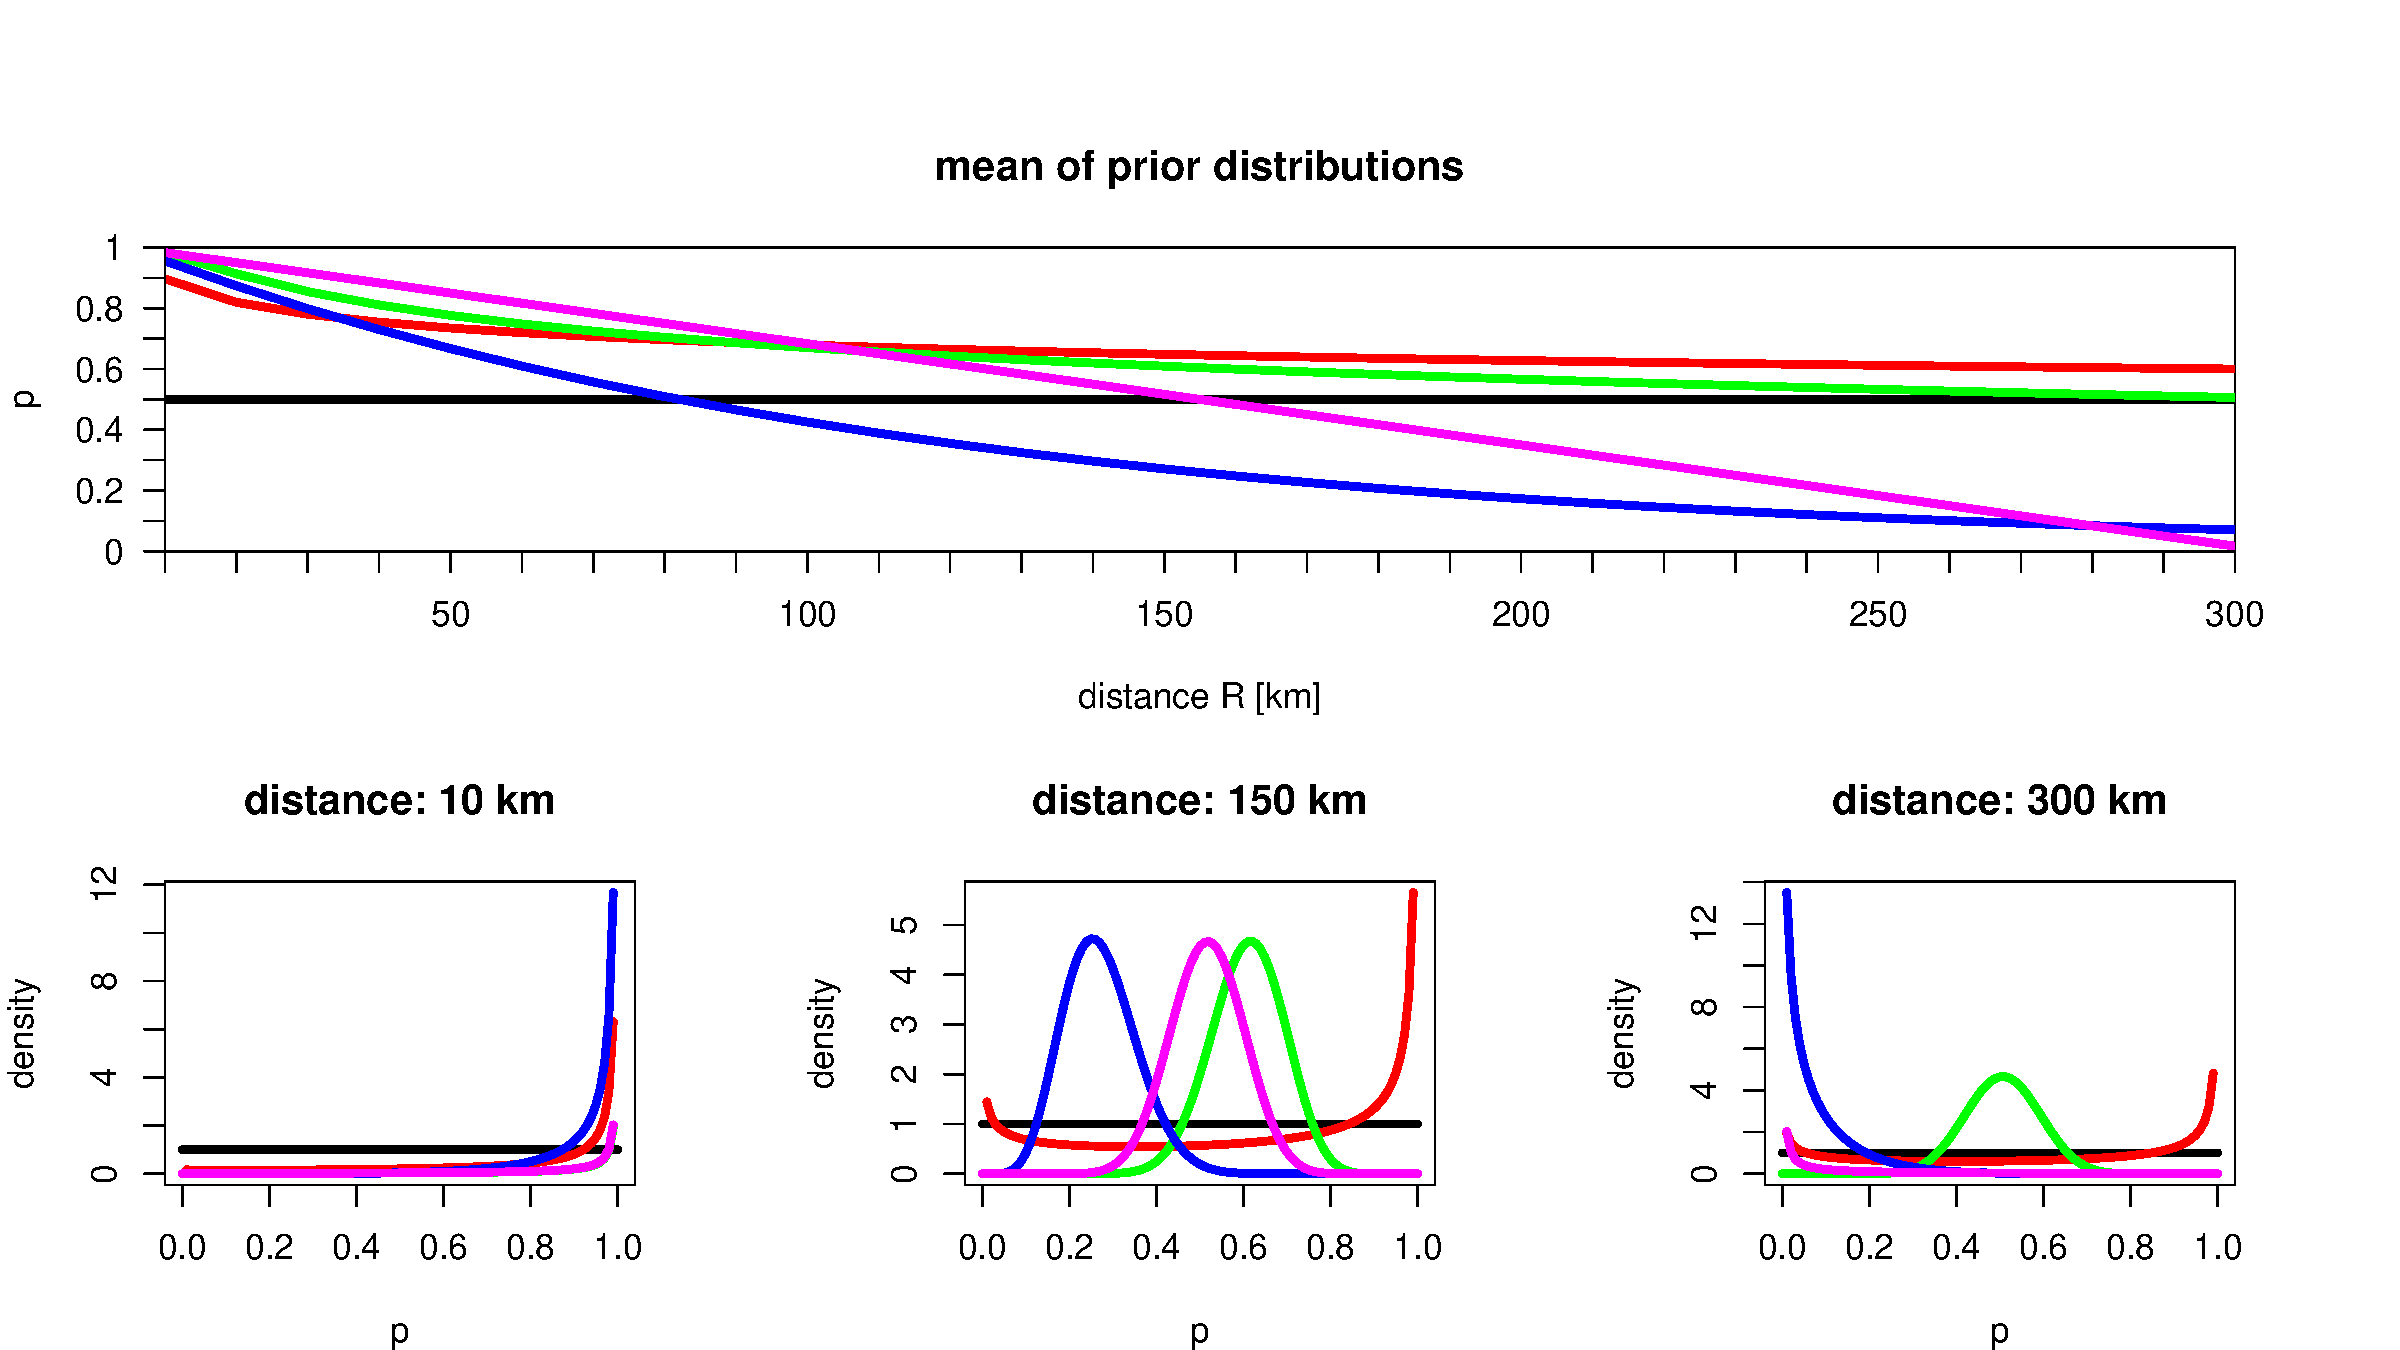
\includegraphics[scale=0.35]{Figures/priorMeans.pdf}
		\rule{35em}{0.5pt}
	\caption[prior]{priorMeans}
	\label{fig:priorMeans}
\end{figure}



\begin{figure}[!htpb]
    \centering
		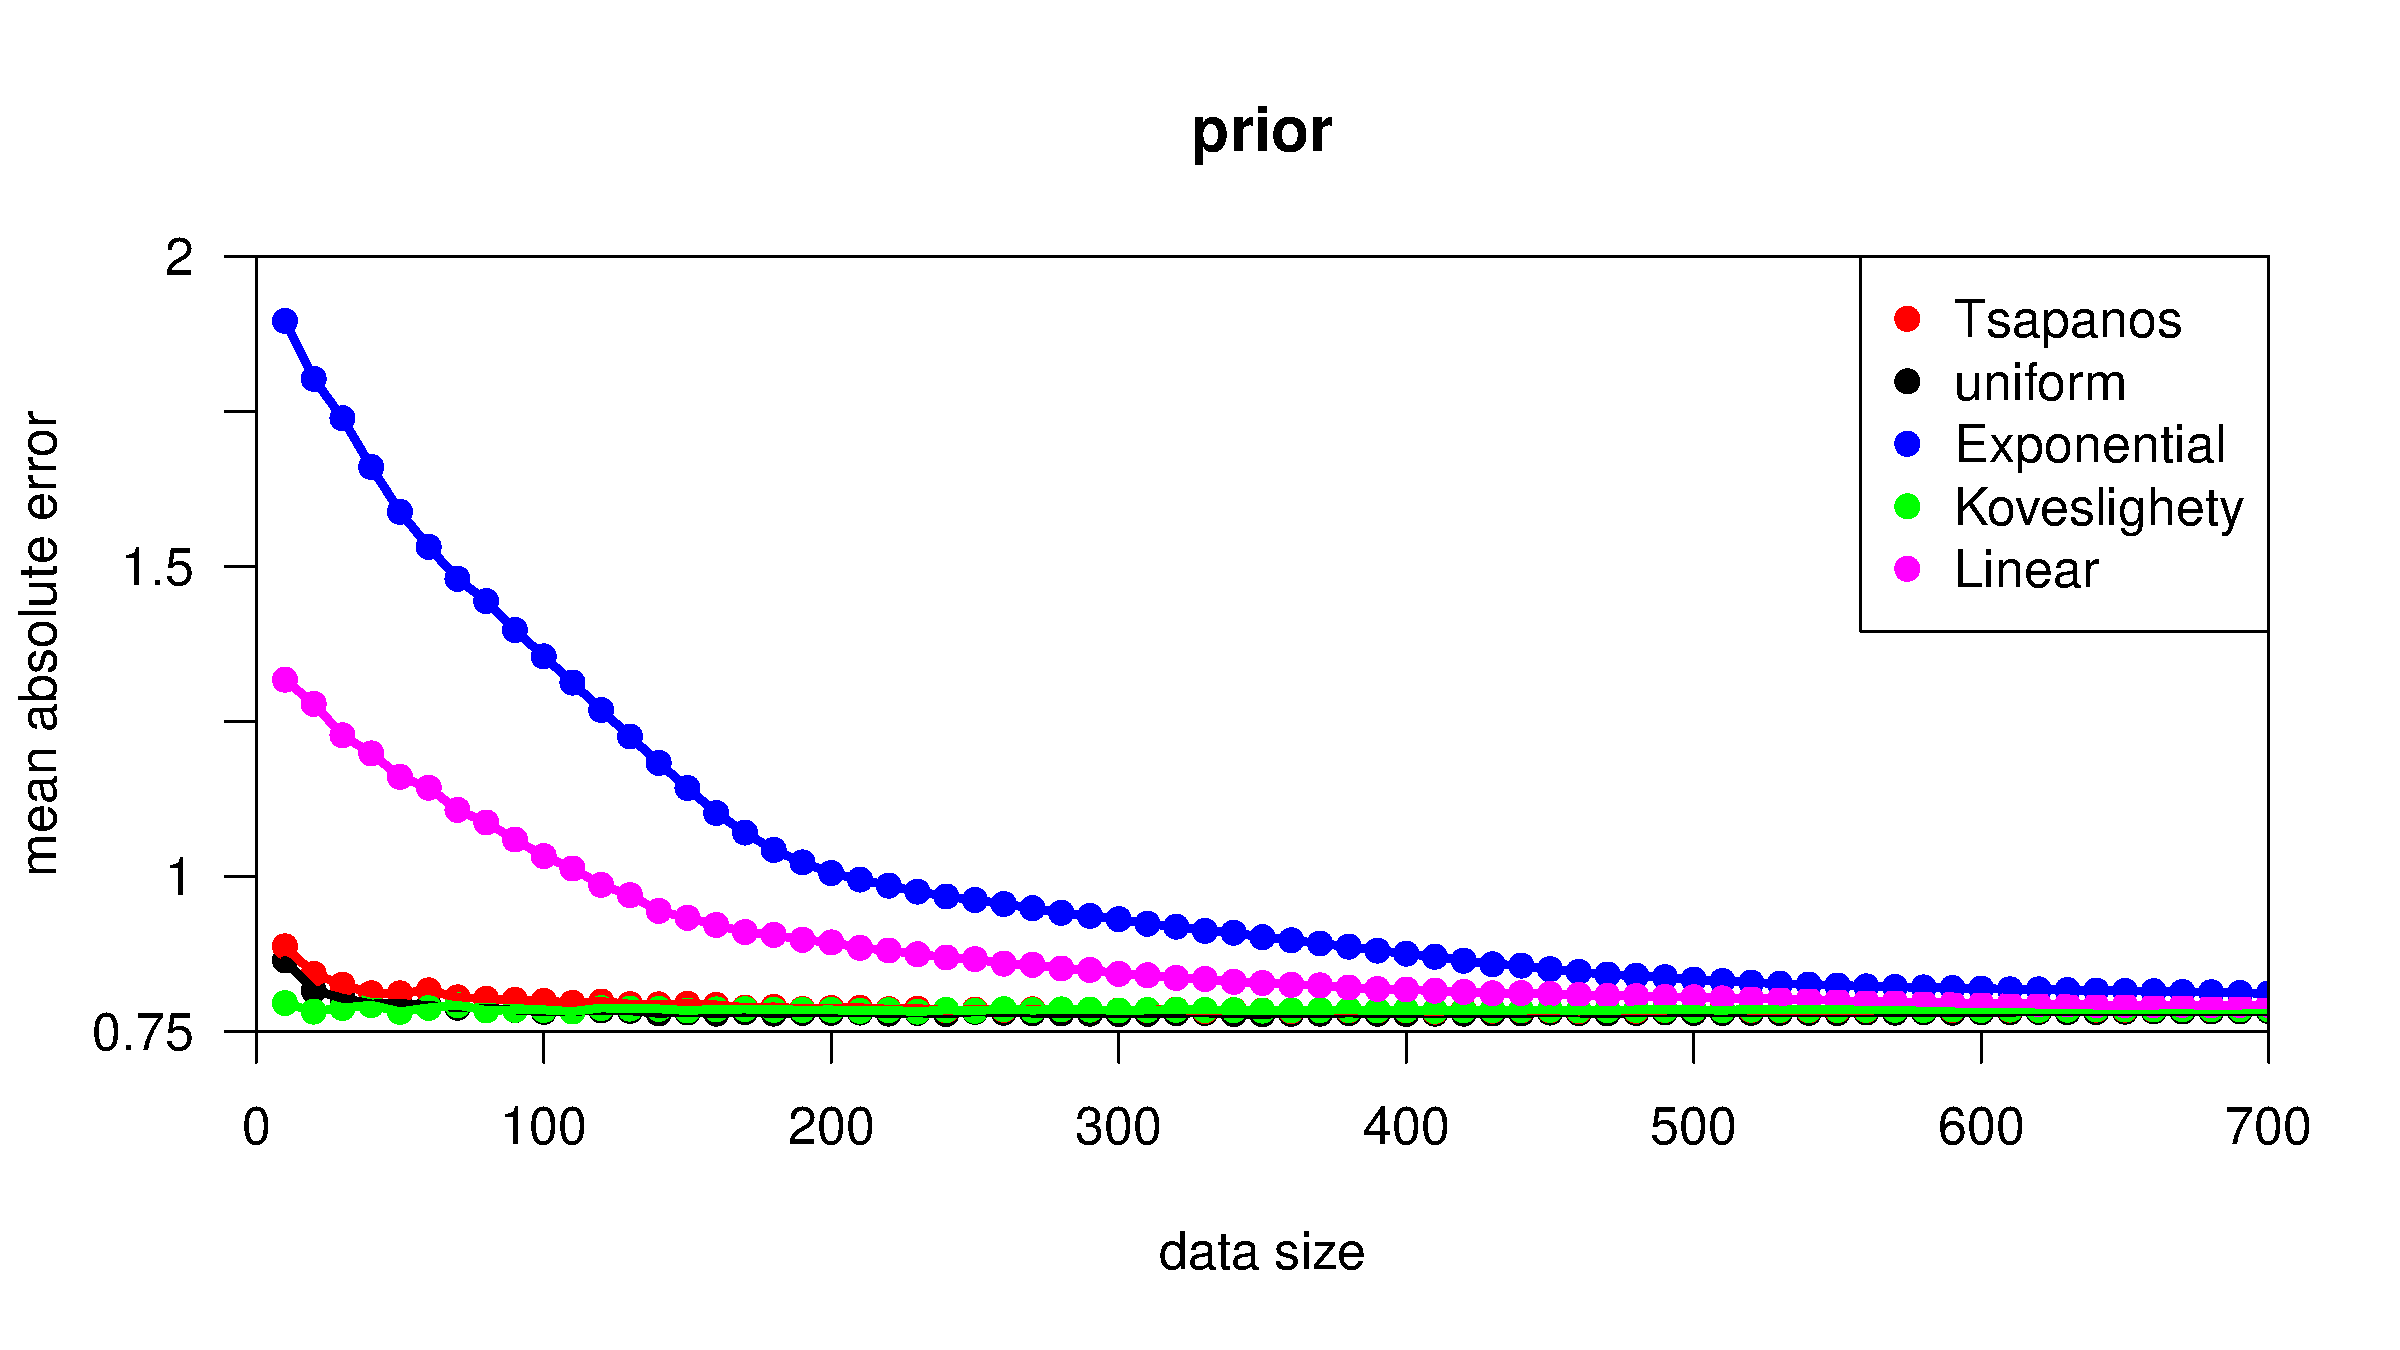
\includegraphics[scale=0.33]{Figures/prior.pdf}
		\rule{35em}{0.5pt}
	\caption[prior]{prior}
	\label{fig:prior}
\end{figure}



\section{Extended Source}


\begin{subequations}
\begin{equation}
\begin{aligned}
&x_1 = x\\ 
& y_1 = y
\end{aligned}
\end{equation}
\begin{equation}
\begin{aligned}
&x_2 = cos(-\theta)*x_1-sin(-\theta)*y_1 \\
&y_2 = sin(-\theta)*x_1+cos(-\theta)*y_1 \\
\end{aligned}
\end{equation}
\begin{equation}
\begin{aligned}
&x_3 = x_2 * \dfrac{b}{a} \\
&y_3 = y_2\\
\end{aligned}
\end{equation}
\begin{equation}
\begin{aligned}
&\gamma = atan(\dfrac{y_3}{x_3} )-atan(\dfrac{y_2}{x_2} )+abs(\theta)\\
&x_4 = cos(\gamma)*x_3-sin(\gamma)*y_3\\
&y_4 = sin(\gamma)*x_3+cos(\gamma)*y_3
\end{aligned}
\end{equation}
\label{eqn:transformR}
\end{subequations}

\begin{figure}[!htpb]
    \centering
		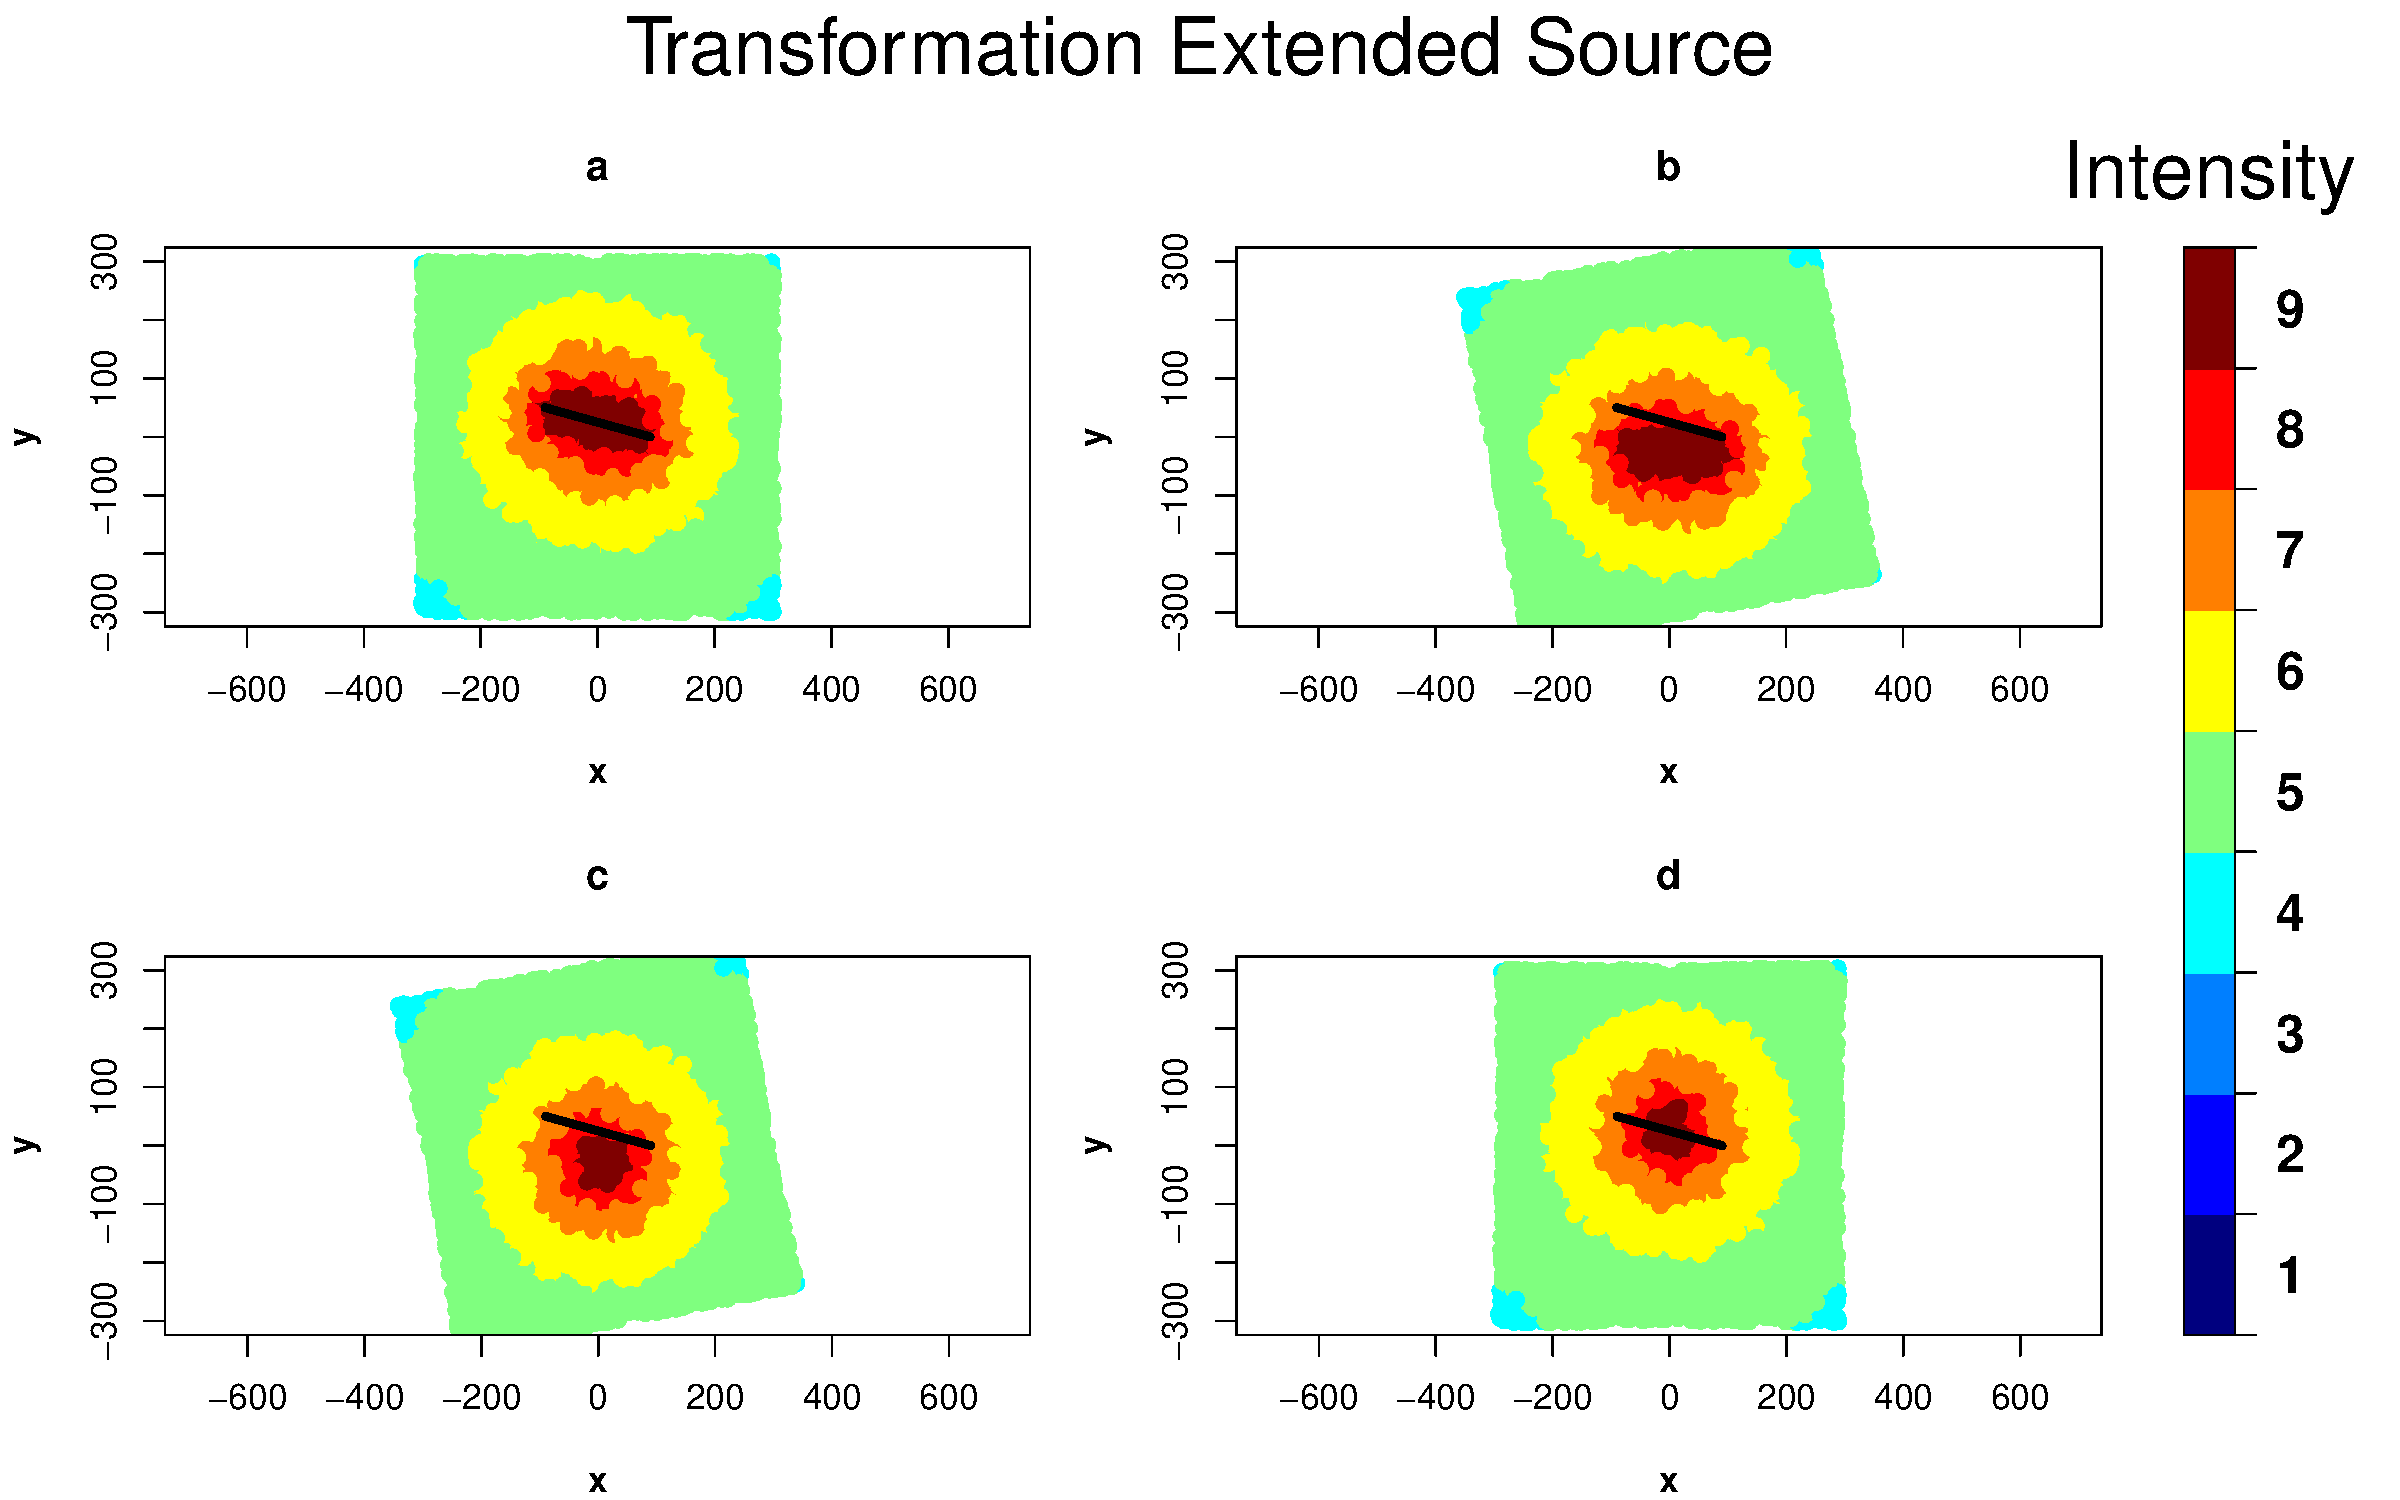
\includegraphics[scale=0.35]{Figures/extendedSource.pdf}
		\rule{35em}{0.5pt}
	\caption[extended Source]{extended Source}
	\label{fig:extendedSource}
\end{figure}

Results: 0.1551224 0.2623517 
% Chapter 4

\chapter{Case Study} % Main chapter title

\label{Chapter4} % For referencing the chapter elsewhere, use \ref{Chapter1} 

\lhead{4. \emph{Case Study}} % This is for the header on each page - perhaps a shortened title

\begin{figure}[!htpb]
	\centering
		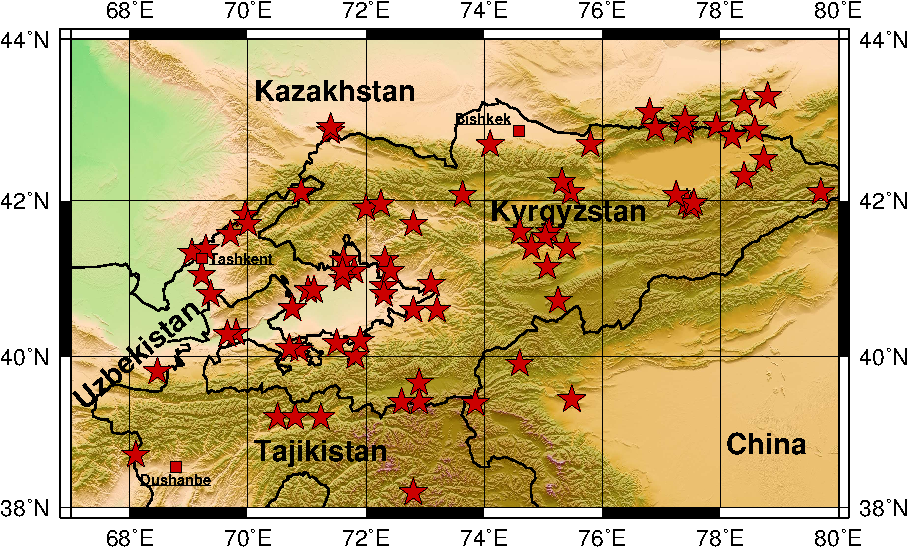
\includegraphics[scale=0.9]{Figures/CentralAsia.pdf}
		\rule{35em}{0.5pt}
	\caption[map]{map}
	\label{fig:map}
\end{figure}

\section{Data}


\begin{table}[ht]
  \centering
        \small
        \setlength\tabcolsep{2pt}
\begin{tabular}{|r|r|r|r|r|r|r|r|r|r|r|r|r|r|r|r|r||r|}
  \hline
$I_0 / I_s$ & 1.5 & 2 & 2.5 & 3 & 3.5 & 4 & 4.5 & 5 & 5.5 & 6 & 6.5 & 7 & 7.5 & 8 & 8.5 & 9 & total \\ 
  \hline
9 & 0 & 0 & 0 & 0 & 13 & 4 & 25 & 23 & 34 & 15 & 23 & 13 & 17 & 4 & 13 & 3 & 187 \\ 
  8.5 & 0 & 0 & 11 & 10 & 62 & 13 & 142 & 33 & 147 & 25 & 153 & 90 & 98 & 14 & 110 & 0 & 908 \\ 
  8 & 0 & 0 & 24 & 9 & 24 & 8 & 48 & 18 & 47 & 28 & 26 & 10 & 9 & 5 & 0 & 0 & 256 \\ 
  7.5 & 3 & 16 & 33 & 68 & 198 & 186 & 204 & 133 & 116 & 76 & 91 & 23 & 24 & 0 & 0 & 0 & 1171 \\ 
  7 & 4 & 24 & 69 & 75 & 149 & 132 & 139 & 67 & 79 & 29 & 29 & 9 & 0 & 0 & 0 & 0 & 805 \\ 
  6.5 & 1 & 15 & 104 & 98 & 219 & 146 & 129 & 60 & 118 & 71 & 56 & 0 & 0 & 0 & 0 & 0 & 1017 \\ 
  6 & 17 & 26 & 103 & 131 & 189 & 86 & 105 & 64 & 90 & 34 & 0 & 0 & 0 & 0 & 0 & 0 & 845 \\ 
  5.5 & 0 & 22 & 155 & 116 & 233 & 166 & 147 & 46 & 70 & 0 & 0 & 0 & 0 & 0 & 0 & 0 & 955 \\ 
  5 & 8 & 1 & 9 & 23 & 19 & 7 & 5 & 5 & 0 & 0 & 0 & 0 & 0 & 0 & 0 & 0 & 77 \\ 
  \hline
  total & 33 & 104 & 508 & 530 & 1106 & 748 & 944 & 449 & 701 & 278 & 378 & 145 & 148 & 23 & 123 & 3 & 6221 \\ 
   \hline
\end{tabular}
\caption[Data]{Data}
\label{table:Data}
\end{table}

\section{Handling uncertain data}

sdavasgas
\begin{table}[ht]
\centering
\begin{tabular}{rrrrrrr}
  \hline
 $I_0$& round & floor & ceiling & Certain & Inflated & Inflated Uncertain \\ 
  \hline 
  5 & - & \cellcolor{green!25}0.493506 & - & - & 0.571429 & \cellcolor{red!25}0.584416 \\ 
  6 & 0.553543 & 0.541667 & \cellcolor{green!25}0.496124 & 0.489256 & 0.566914 & \cellcolor{red!25}0.584479 \\ 
  7 & 0.660767 & \cellcolor{green!25}0.656970 & 0.677229 & 0.681021 & \cellcolor{red!25}0.695033 & 0.679183 \\ 
  8 & 0.556452 & \cellcolor{green!25}0.504555 & \cellcolor{red!25}0.601721 & 0.521674 & 0.593300 & 0.544509 \\ 
  9 & 0.748899 & 0.743379 & \cellcolor{red!25}0.816151 & \cellcolor{green!25}0.697095 & 0.807437 & 0.787307 \\ 
  10 & \cellcolor{red!25}0.620321 & - & \cellcolor{green!25}0.582888 &-  & 0.604278 & 0.614973 \\ 
   \hline
\end{tabular}
\caption[Data]{Data}
     \label{table:Rotondi}
\end{table}

\section{Comparison to other studies}


\begin{table}[!ht]
\centering
\begin{tabular}{rrr}
  \hline
 $I_0$& Rotondi & Ullah \\ 
  \hline
  5 & \cellcolor{green!25}0.493506  & \cellcolor{red!25}0.934634\\ 
  6 & \cellcolor{green!25} 0.541667 & \cellcolor{red!25}0.613935 \\ 
  7 & \cellcolor{green!25}0.656970  & \cellcolor{red!25}0.570863 \\ 
  8 & \cellcolor{green!25}0.504555 & \cellcolor{red!25}0.562258  \\ 
  9 & \cellcolor{red!25}0.743379 & \cellcolor{green!25}0.743313  \\ 
  10 & - & - \\ 
   \hline
   \end{tabular}
\caption[Data]{Data}
     \label{table:Ullah}
\end{table}

\section{Extended Source}
% Chapter 5

\chapter{Conclusions} % Main chapter title

\label{Chapter5} % For referencing the chapter elsewhere, use \ref{Chapter1} 

\lhead{4. \emph{Conclusions}} % This is for the header on each page - perhaps a shortened title


Conclusions:
what did you find out?
general advises
outlook 
 
%\input{Chapters/Chapter6} 
%\input{Chapters/Chapter7} 

%----------------------------------------------------------------------------------------
%	THESIS CONTENT - APPENDICES
%----------------------------------------------------------------------------------------

\addtocontents{toc}{\vspace{2em}} % Add a gap in the Contents, for aesthetics

\appendix % Cue to tell LaTeX that the following 'chapters' are Appendices

% Include the appendices of the thesis as separate files from the Appendices folder
% Uncomment the lines as you write the Appendices

% Appendix Template

\chapter{Data} % Main appendix title

\label{AppendixA} % Change X to a consecutive letter; for referencing this appendix elsewhere, use \ref{AppendixX}

\lhead{Appendix A. \emph{Data}} % Change X to a consecutive letter; this is for the header on each page - perhaps a shortened title


  
\setlength\tabcolsep{2pt}\small        
\begin{longtable}{cccccccccccccccccc}
\centering
 & year & month & day & $\lambda$ & $\theta$ & $\phi$ & $I_{max}$ & depth & K & MLH & $M_W$ & Length & F1.1 & F1.2 & F2.1 & F2.2 \\ 
  \hline
\hline
\endfirsthead
%\multicolumn{4}{c}%
%{\tablename\ \thetable\ -- \textit{Continued from previous page}} \\
\hline
 & year & month & day & $\lambda$ & $\theta$& $\phi$ & $I_{max}$ & depth  & K & MLH & $M_W$ & Length & F1.1 & F1.2 & F2.1 & F2.2 \\ 
  \hline 
\hline
\endhead
\hline %\multicolumn{4}{r}{\textit{Continued on next page}} \\
\endfoot
\endlastfoot
1 & 1883 & 11 & 14 & 72.80 & 40.60 & 200 & 7 & 12 & 13.9 & 5.383 & 5.68 & 4.98 & 72.790 & 40.579 & 72.823 & 40.586 \\ 
  2 & 1885 & 8 & 2 & 74.10 & 42.70 & 250 & 9 & 15 & 15.6 & 6.182 & 6.20 & 11.43 & 74.034 & 42.682 & 74.155 & 42.668 \\ 
  3 & 1887 & 6 & 8 & 76.80 & 43.10 & 250 & 9 & 20 & 16.9 & 6.793 & 6.81 & 29.89 & 76.627 & 43.054 & 76.945 & 43.017 \\ 
  4 & 1889 & 7 & 11 & 78.40 & 43.20 & 250 & 9 & 40 & 18.5 & 7.545 & 7.55 & 97.54 & 77.837 & 43.049 & 78.872 & 42.929 \\ 
  5 & 1897 & 9 & 17 & 68.47 & 39.80 & 270 & 8 & 25 & 15.4 & 6.088 & 6.15 & 10.54 & 68.405 & 39.800 & 68.515 & 39.771 \\ 
  6 & 1902 & 12 & 16 & 72.30 & 40.80 & 270 & 9 & 9 & 15.6 & 6.182 & 6.20 & 11.43 & 72.232 & 40.800 & 72.353 & 40.768 \\ 
  7 & 1907 & 10 & 21 & 68.10 & 38.70 & 270 & 9 & 24 & 17.0 & 6.840 & 6.85 & 32.18 & 67.915 & 38.700 & 68.246 & 38.611 \\ 
  8 & 1911 & 1 & 3 & 76.90 & 42.90 & 250 & 10 & 25 & 17.8 & 7.216 & 7.22 & 58.14 & 76.566 & 42.810 & 77.180 & 42.739 \\ 
  9 & 1911 & 2 & 18 & 72.80 & 38.20 & 200 & 9 & 26 & 17.3 & 6.981 & 6.99 & 40.17 & 72.722 & 38.030 & 72.981 & 38.089 \\ 
  10 & 1924 & 7 & 12 & 73.20 & 40.60 & 270 & 8 & 14 & 15.6 & 6.182 & 6.20 & 11.43 & 73.132 & 40.600 & 73.253 & 40.568 \\ 
  11 & 1927 & 8 & 12 & 71.60 & 41.00 & 270 & 8 & 14 & 14.8 & 5.806 & 5.96 & 7.81 & 71.554 & 41.000 & 71.637 & 40.978 \\ 
  12 & 1932 & 12 & 24 & 78.20 & 42.80 & 250 & 6 & 23 & 14.0 & 5.430 & 5.71 & 5.23 & 78.170 & 42.792 & 78.225 & 42.786 \\ 
  13 & 1933 & 9 & 9 & 70.70 & 40.10 & 270 & 6 & 26 & 13.6 & 5.242 & 5.58 & 4.28 & 70.675 & 40.100 & 70.720 & 40.088 \\ 
  14 & 1937 & 12 & 18 & 70.90 & 42.10 & 270 & 7 & 25 & 15.6 & 6.182 & 6.20 & 11.43 & 70.831 & 42.100 & 70.955 & 42.068 \\ 
  15 & 1938 & 6 & 20 & 75.80 & 42.70 & 250 & 8 & 21 & 16.0 & 6.370 & 6.39 & 15.37 & 75.712 & 42.676 & 75.874 & 42.657 \\ 
  16 & 1941 & 4 & 20 & 70.50 & 39.20 & 270 & 9 & 8 & 15.6 & 6.182 & 6.20 & 11.43 & 70.434 & 39.200 & 70.552 & 39.168 \\ 
  17 & 1942 & 1 & 18 & 71.60 & 41.10 & 270 & 7 & 21 & 14.0 & 5.430 & 5.71 & 5.23 & 71.569 & 41.100 & 71.625 & 41.086 \\ 
  18 & 1946 & 11 & 2 & 72.00 & 41.90 & 270 & 9 & 25 & 17.0 & 6.840 & 6.85 & 32.18 & 71.806 & 41.900 & 72.153 & 41.811 \\ 
  19 & 1947 & 6 & 2 & 72.30 & 40.90 & 270 & 8 & 13 & 14.5 & 5.665 & 5.87 & 6.72 & 72.260 & 40.900 & 72.331 & 40.881 \\ 
  20 & 1948 & 7 & 28 & 75.40 & 41.40 & 250 & 7 & 6 & 13.6 & 5.242 & 5.58 & 4.28 & 75.376 & 41.393 & 75.420 & 41.388 \\ 
  21 & 1949 & 7 & 10 & 70.80 & 39.20 & 200 & 9 & 16 & 17.0 & 6.840 & 6.85 & 32.18 & 70.736 & 39.064 & 70.947 & 39.111 \\ 
  22 & 1954 & 12 & 3 & 74.80 & 41.40 & 250 & 7 & 15 & 14.0 & 5.430 & 5.71 & 5.23 & 74.771 & 41.392 & 74.825 & 41.386 \\ 
  23 & 1955 & 4 & 15 & 74.60 & 39.90 & 200 & 9 & 25 & 16.4 & 6.558 & 6.57 & 20.65 & 74.559 & 39.813 & 74.695 & 39.843 \\ 
  24 & 1957 & 5 & 8 & 74.60 & 41.60 & 250 & 6 & 7 & 13.0 & 4.960 & 5.39 & 3.17 & 74.582 & 41.595 & 74.615 & 41.591 \\ 
  25 & 1958 & 10 & 13 & 75.10 & 41.60 & 250 & 6 & 12 & 13.0 & 4.960 & 5.39 & 3.17 & 75.082 & 41.595 & 75.115 & 41.591 \\ 
  26 & 1959 & 7 & 12 & 72.80 & 41.70 & 270 & 6 & 14 & 12.9 & 4.913 & 5.36 & 3.02 & 72.782 & 41.700 & 72.814 & 41.692 \\ 
  27 & 1959 & 10 & 24 & 70.00 & 41.70 & 270 & 7 & 13 & 14.0 & 5.430 & 5.71 & 5.23 & 69.969 & 41.700 & 70.025 & 41.686 \\ 
  28 & 1960 & 12 & 18 & 78.40 & 42.30 & 250 & 6 & 17 & 12.8 & 4.866 & 5.33 & 2.87 & 78.384 & 42.296 & 78.414 & 42.292 \\ 
  29 & 1961 & 4 & 27 & 72.90 & 39.65 & 200 & 6 & 26 & 14.2 & 5.524 & 5.77 & 5.78 & 72.888 & 39.626 & 72.927 & 39.634 \\ 
  30 & 1962 & 9 & 3 & 73.10 & 40.93 & 270 & 7 & 20 & 14.0 & 5.430 & 5.71 & 5.23 & 73.069 & 40.933 & 73.125 & 40.919 \\ 
  31 & 1963 & 10 & 19 & 71.62 & 41.23 & 270 & 6 & 8 & 12.5 & 4.725 & 5.24 & 2.47 & 71.602 & 41.233 & 71.628 & 41.227 \\ 
  32 & 1965 & 3 & 17 & 69.37 & 40.80 & 270 & 7 & 12 & 13.0 & 4.960 & 5.39 & 3.17 & 69.348 & 40.800 & 69.381 & 40.791 \\ 
  33 & 1965 & 9 & 25 & 75.03 & 41.53 & 250 & 6 & 25 & 13.0 & 4.960 & 5.39 & 3.17 & 75.015 & 41.528 & 75.048 & 41.525 \\ 
  34 & 1965 & 10 & 18 & 77.55 & 41.97 & 250 & 6 & 15 & 13.0 & 4.960 & 5.39 & 3.17 & 77.532 & 41.962 & 77.565 & 41.958 \\ 
  35 & 1966 & 4 & 25 & 69.28 & 41.38 & 270 & 6 & 8 & 13.3 & 5.101 & 5.49 & 3.69 & 69.261 & 41.383 & 69.301 & 41.373 \\ 
  36 & 1966 & 4 & 30 & 71.80 & 41.10 & 270 & 6 & 20 & 13.6 & 5.242 & 5.58 & 4.28 & 71.774 & 41.100 & 71.820 & 41.088 \\ 
  37 & 1967 & 5 & 18 & 70.75 & 40.62 & 270 & 6 & 25 & 12.0 & 4.490 & 5.08 & 1.92 & 70.739 & 40.617 & 70.759 & 40.611 \\ 
  38 & 1967 & 9 & 28 & 79.70 & 42.10 & 250 & 6 & 18 & 13.5 & 5.195 & 5.55 & 4.07 & 79.677 & 42.094 & 79.719 & 42.089 \\ 
  39 & 1967 & 11 & 30 & 77.40 & 43.00 & 250 & 6 & 10 & 12.0 & 4.490 & 5.08 & 1.92 & 77.389 & 42.997 & 77.409 & 42.995 \\ 
  40 & 1968 & 3 & 20 & 75.07 & 41.15 & 250 & 6 & 17 & 12.6 & 4.772 & 5.27 & 2.60 & 75.052 & 41.146 & 75.079 & 41.143 \\ 
  41 & 1970 & 1 & 19 & 69.22 & 41.05 & 270 & 7 & 25 & 12.1 & 4.537 & 5.11 & 2.02 & 69.205 & 41.050 & 69.226 & 41.044 \\ 
  42 & 1970 & 6 & 5 & 78.73 & 42.52 & 250 & 8 & 15 & 15.6 & 6.182 & 6.20 & 11.43 & 78.668 & 42.499 & 78.788 & 42.485 \\ 
  43 & 1971 & 5 & 10 & 71.40 & 42.92 & 250 & 7 & 20 & 14.0 & 5.430 & 5.71 & 5.23 & 71.370 & 42.909 & 71.425 & 42.902 \\ 
  44 & 1971 & 10 & 28 & 72.25 & 41.95 & 270 & 6 & 17 & 14.0 & 5.430 & 5.71 & 5.23 & 72.218 & 41.950 & 72.275 & 41.936 \\ 
  45 & 1972 & 3 & 17 & 69.65 & 40.28 & 270 & 6 & 20 & 13.5 & 5.195 & 5.55 & 4.07 & 69.626 & 40.283 & 69.669 & 40.272 \\ 
  46 & 1974 & 1 & 22 & 71.90 & 40.20 & 270 & 7 & 24 & 12.7 & 4.819 & 5.30 & 2.73 & 71.884 & 40.200 & 71.913 & 40.192 \\ 
  47 & 1974 & 2 & 20 & 75.25 & 40.72 & 250 & 6 & 15 & 13.2 & 5.054 & 5.46 & 3.51 & 75.230 & 40.711 & 75.266 & 40.707 \\ 
  48 & 1974 & 7 & 2 & 75.32 & 42.23 & 250 & 6 & 15 & 12.9 & 4.913 & 5.36 & 3.02 & 75.299 & 42.229 & 75.331 & 42.225 \\ 
  49 & 1974 & 8 & 11 & 73.85 & 39.38 & 200 & 6 & 15 & 16.6 & 6.652 & 6.67 & 23.94 & 73.802 & 39.282 & 73.960 & 39.317 \\ 
  50 & 1975 & 2 & 12 & 78.80 & 43.30 & 250 & 6 & 10 & 13.0 & 4.960 & 5.39 & 3.17 & 78.782 & 43.295 & 78.815 & 43.291 \\ 
  51 & 1977 & 1 & 31 & 70.87 & 40.08 & 296 & 8 & 20 & 15.5 & 6.135 & 6.15 & 10.62 & 70.811 & 40.104 & 70.916 & 40.054 \\ 
  52 & 1977 & 6 & 3 & 71.82 & 40.00 & 128 & 6 & 15 & 14.2 & 5.524 & 5.77 & 5.78 & 71.843 & 39.984 & 71.843 & 39.984 \\ 
  53 & 1977 & 12 & 6 & 69.70 & 41.57 & 270 & 7 & 15 & 14.0 & 5.430 & 5.71 & 5.23 & 69.669 & 41.567 & 69.725 & 41.552 \\ 
  54 & 1978 & 3 & 24 & 78.58 & 42.88 & 270 & 8 & 22 & 15.6 & 6.182 & 6.20 & 11.43 & 78.513 & 42.883 & 78.639 & 42.852 \\ 
  55 & 1978 & 11 & 1 & 72.60 & 39.40 & 200 & 8 & 30 & 16.2 & 6.464 & 6.48 & 17.81 & 72.565 & 39.325 & 72.682 & 39.351 \\ 
  56 & 1979 & 4 & 6 & 77.43 & 41.97 & 121 & 6 & 25 & 13.5 & 5.195 & 5.55 & 4.07 & 77.454 & 41.957 & 77.453 & 41.955 \\ 
  57 & 1980 & 7 & 5 & 77.50 & 41.92 & 250 & 6 & 20 & 13.8 & 5.336 & 5.65 & 4.73 & 77.473 & 41.909 & 77.523 & 41.904 \\ 
  58 & 1980 & 12 & 11 & 69.05 & 41.33 & 270 & 7 & 10 & 13.5 & 5.195 & 5.55 & 4.07 & 69.026 & 41.333 & 69.069 & 41.322 \\ 
  59 & 1982 & 5 & 6 & 71.50 & 40.17 & 112 & 8 & 20 & 14.4 & 5.618 & 5.83 & 6.39 & 71.535 & 40.156 & 71.530 & 40.149 \\ 
  60 & 1982 & 12 & 31 & 77.37 & 42.87 & 274 & 6 & 15 & 13.6 & 5.242 & 5.58 & 4.28 & 77.340 & 42.868 & 77.387 & 42.855 \\ 
  61 & 1983 & 12 & 16 & 72.90 & 39.40 & 228 & 7 & 15 & 14.6 & 5.712 & 5.90 & 7.06 & 72.870 & 39.379 & 72.932 & 39.380 \\ 
  62 & 1983 & 12 & 21 & 77.25 & 42.07 & 250 & 6 & 20 & 12.5 & 4.725 & 5.24 & 2.47 & 77.236 & 42.063 & 77.262 & 42.060 \\ 
  63 & 1984 & 2 & 2 & 71.40 & 42.87 & 250 & 6 & 15 & 12.6 & 4.772 & 5.27 & 2.60 & 71.385 & 42.863 & 71.413 & 42.859 \\ 
  64 & 1984 & 2 & 17 & 71.02 & 40.85 & 240 & 8 & 10 & 14.1 & 5.477 & 5.74 & 5.50 & 70.988 & 40.838 & 71.042 & 40.835 \\ 
  65 & 1984 & 10 & 26 & 71.23 & 39.20 & 37 & 8 & 15 & 14.8 & 5.806 & 5.96 & 7.81 & 71.261 & 39.228 & 71.269 & 39.178 \\ 
  66 & 1985 & 4 & 27 & 71.12 & 40.85 & 103 & 8 & 15 & 12.8 & 4.866 & 5.33 & 2.87 & 71.133 & 40.847 & 71.130 & 40.842 \\ 
  67 & 1985 & 8 & 23 & 75.48 & 39.43 & 308 & 7 & 20 & 16.5 & 6.605 & 6.62 & 22.24 & 75.381 & 39.495 & 75.585 & 39.372 \\ 
  68 & 1985 & 10 & 13 & 69.80 & 40.30 & 48 & 8 & 10 & 14.8 & 5.806 & 5.96 & 7.81 & 69.834 & 40.323 & 69.836 & 40.278 \\ 
  69 & 1987 & 3 & 26 & 69.95 & 41.82 & 203 & 6 & 5 & 13.1 & 5.007 & 5.42 & 3.33 & 69.942 & 41.803 & 69.966 & 41.807 \\ 
  70 & 1988 & 3 & 13 & 75.47 & 42.10 & 250 & 6 & 7 & 12.6 & 4.772 & 5.27 & 2.60 & 75.452 & 42.096 & 75.479 & 42.093 \\ 
  71 & 1988 & 6 & 17 & 77.40 & 42.93 & 29 & 6 & 21 & 12.9 & 4.913 & 5.36 & 3.02 & 77.409 & 42.945 & 77.415 & 42.925 \\ 
  72 & 1988 & 12 & 21 & 72.32 & 41.23 & 270 & 6 & 10 & 12.9 & 4.913 & 5.36 & 3.02 & 72.299 & 41.233 & 72.331 & 41.225 \\ 
  73 & 1990 & 11 & 12 & 77.93 & 42.93 & 211 & 8 & 15 & 15.3 & 6.041 & 6.12 & 10.02 & 77.902 & 42.895 & 77.982 & 42.906 \\ 
  74 & 1992 & 5 & 15 & 72.42 & 41.10 & 270 & 8 & 10 & 15.3 & 6.041 & 6.12 & 10.02 & 72.357 & 41.100 & 72.464 & 41.072 \\ 
  75 & 1992 & 8 & 19 & 73.63 & 42.07 & 250 & 10 & 25 & 17.0 & 6.840 & 6.85 & 32.18 & 73.451 & 42.017 & 73.787 & 41.978 \\ 
  \hline 
  \caption[Data]{Data \citep{HarvardCMT1} \citep{HarvardCMT2}}
     \label{table:Events}
\end{longtable}



\addtocontents{toc}{\vspace{2em}} % Add a gap in the Contents, for aesthetics

\backmatter

%----------------------------------------------------------------------------------------
%	BIBLIOGRAPHY
%----------------------------------------------------------------------------------------

\label{References}

\lhead{\emph{References}} % Change the page header to say "Bibliography"

\bibliographystyle{apa} % Use the "unsrtnat" BibTeX style for formatting the Bibliography

\bibliography{References} % The references (bibliography) information are stored in the file named "Bibliography.bib"

\end{document}  